% !TEX root = dynamicslearning.tex

\section{Numerical experiments}\label{sec:num}
%In order to convince the reader of the usefulness of Theorem \ref{thm}, we report below in Figure \ref{firstnum} one (of several we did) preliminary numerical experiment  indicating the successful recovery by an adaptive algorithm based on \eqref{fdproxy} of a potential function $a$ in a first order model of the type \eqref{fdgradientflow}. More specifically, we performed successive applications of  \eqref{fdproxy} based on an adaptive refinement of a mesh on the positive real line, defining approximating spaces $V$ of continuous piecewise linear functions. The adaptation is lead by a posteriori error estimator based on local comparison of two successive iterations.
%
%
%\begin{figure}[h]
%\begin{center}
% 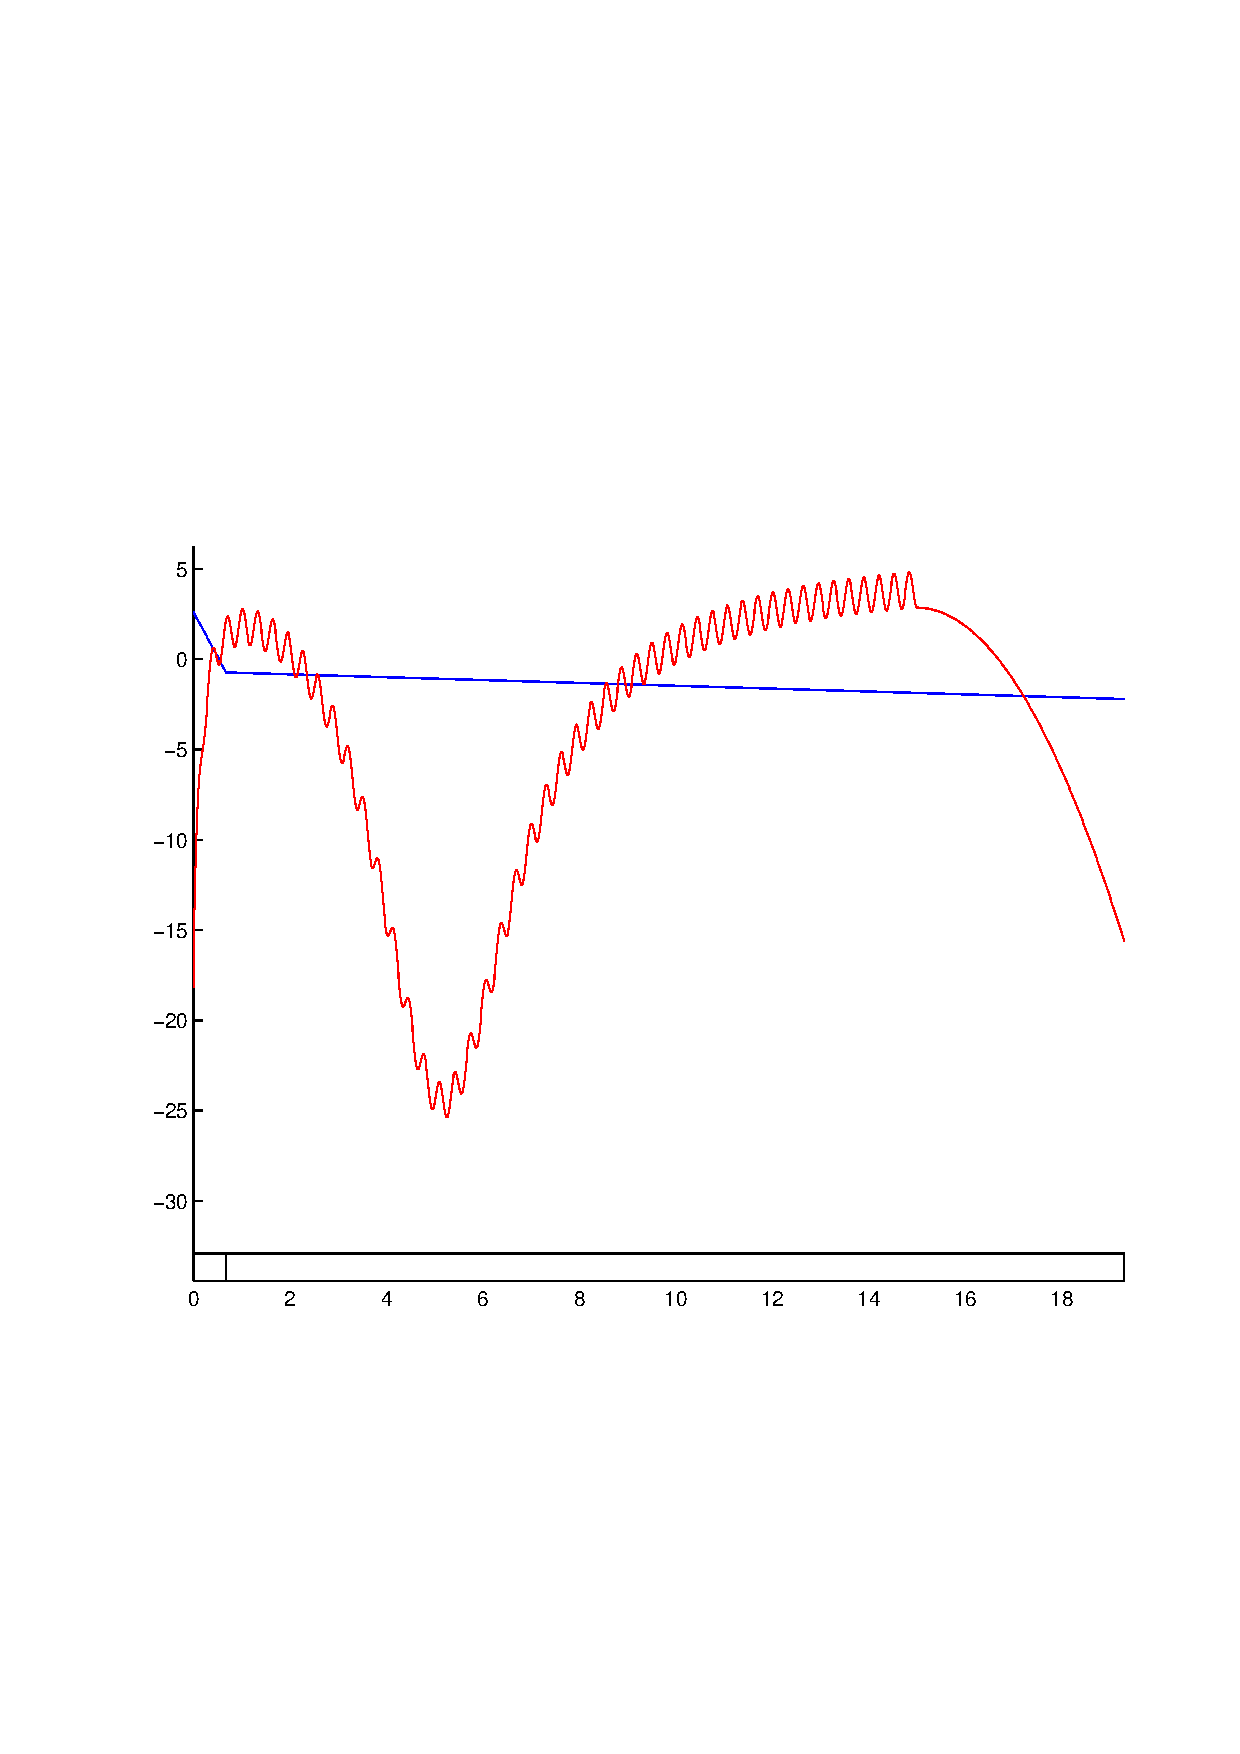
\includegraphics[width=0.3\textwidth]{Figure1}
%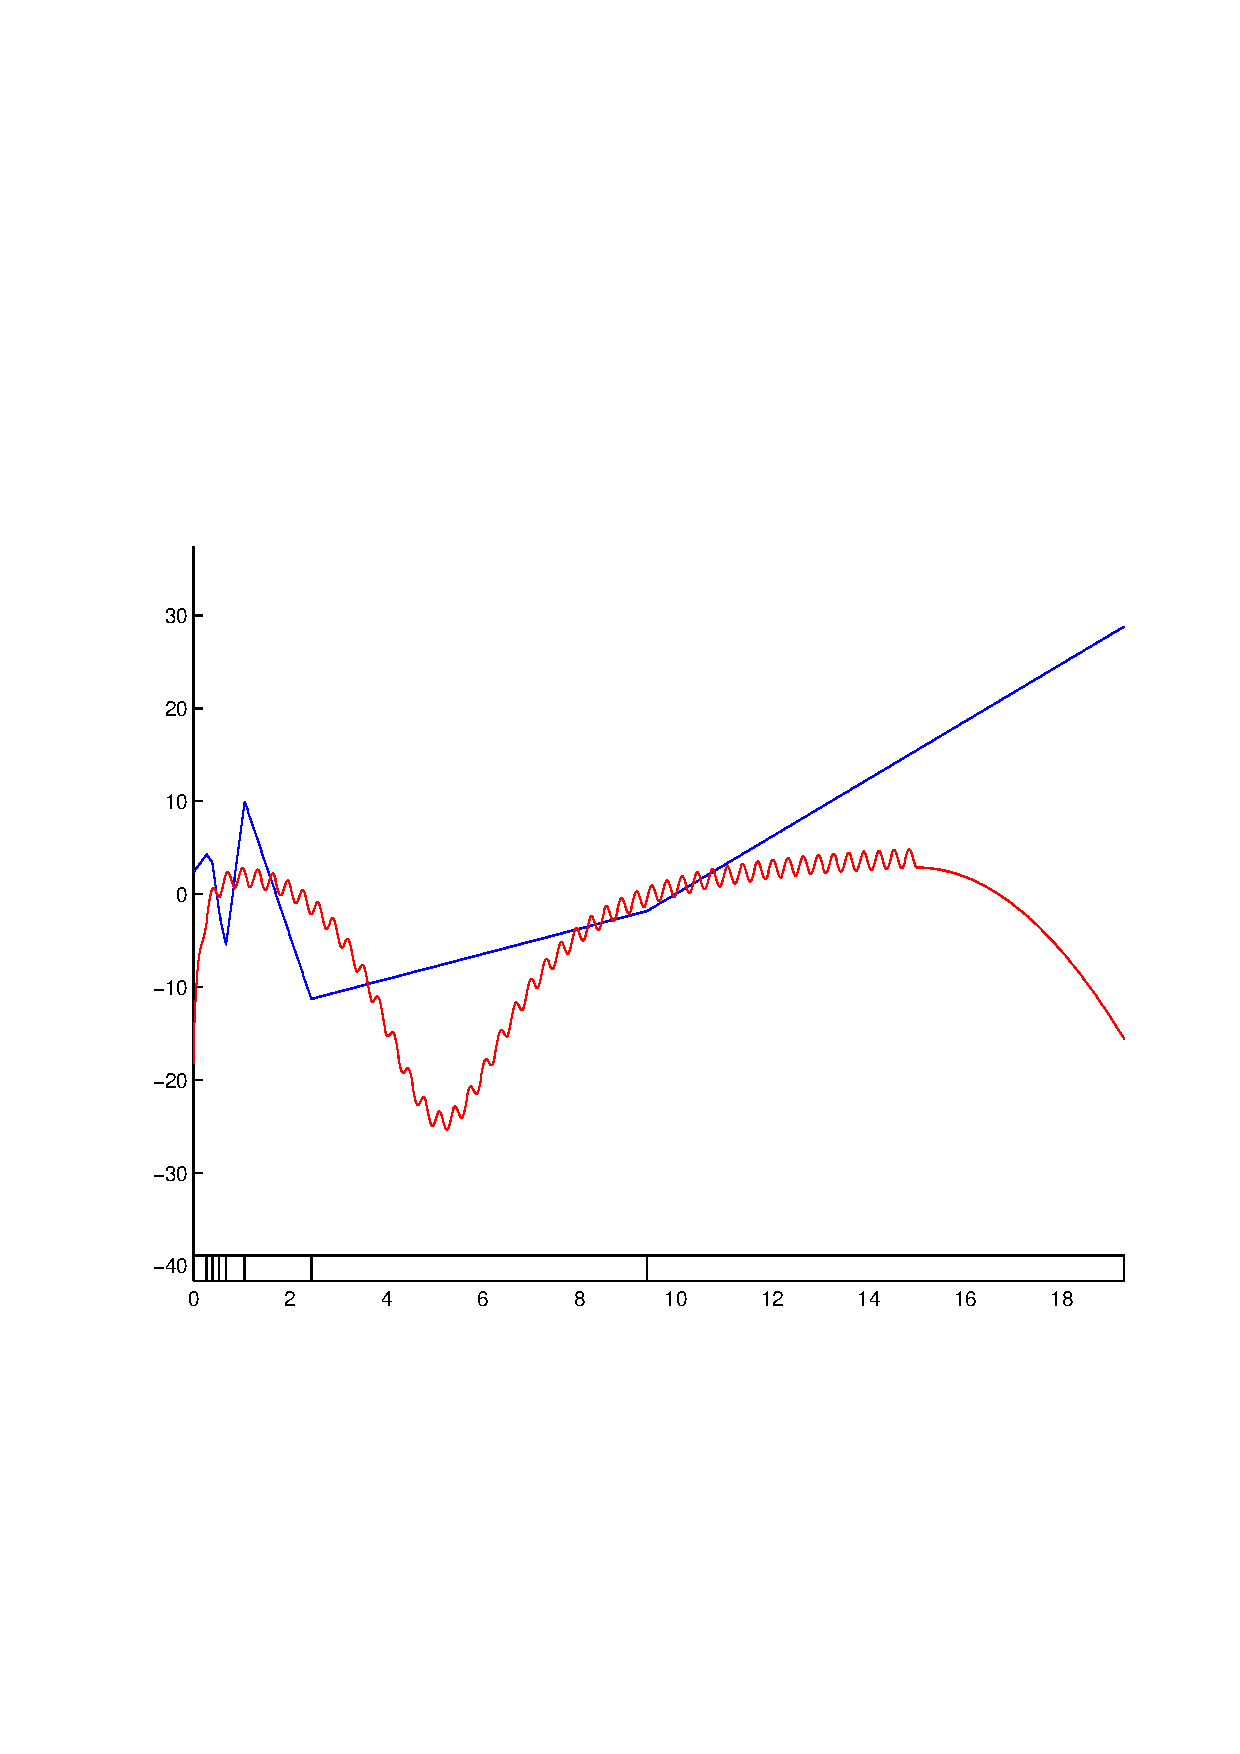
\includegraphics[width=0.3\textwidth]{Figure3}
%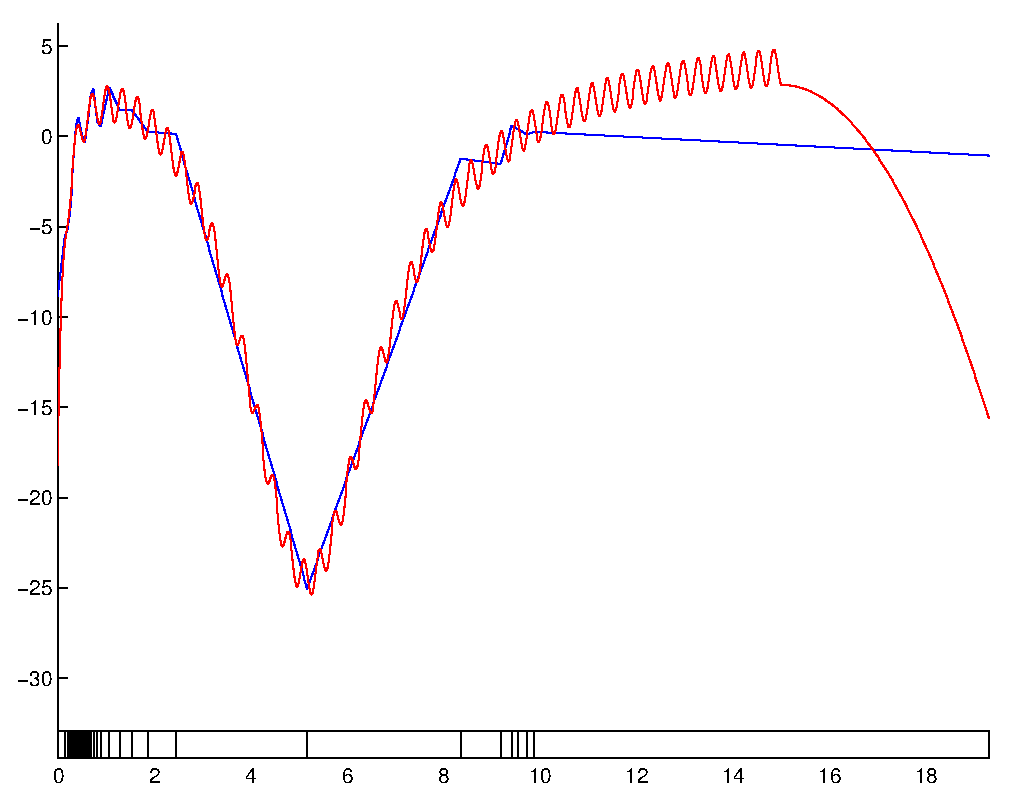
\includegraphics[width=0.3\textwidth]{Figure5}
%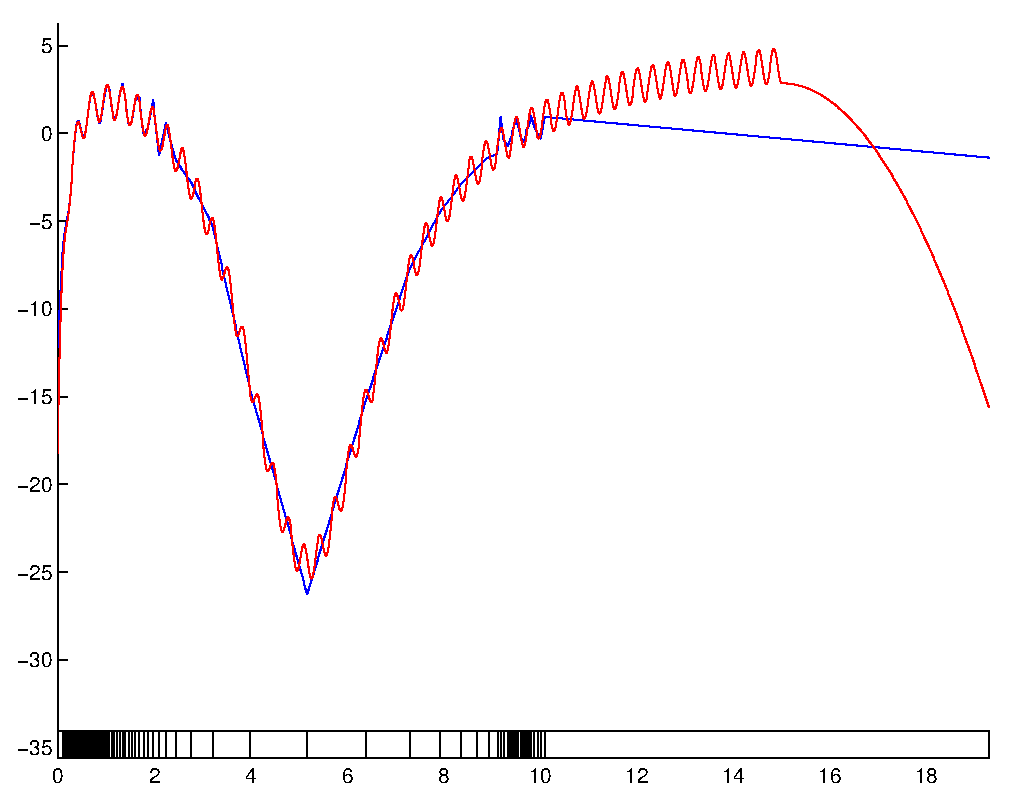
\includegraphics[width=0.3\textwidth]{Figure7}
%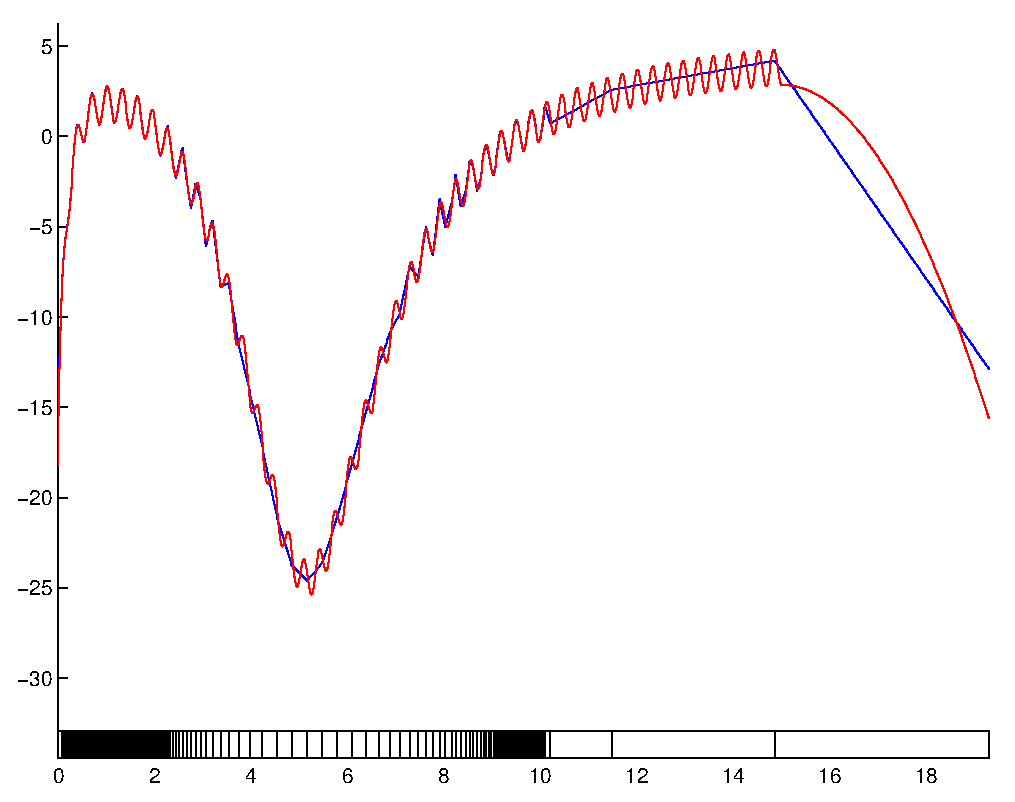
\includegraphics[width=0.3\textwidth]{Figure9}
%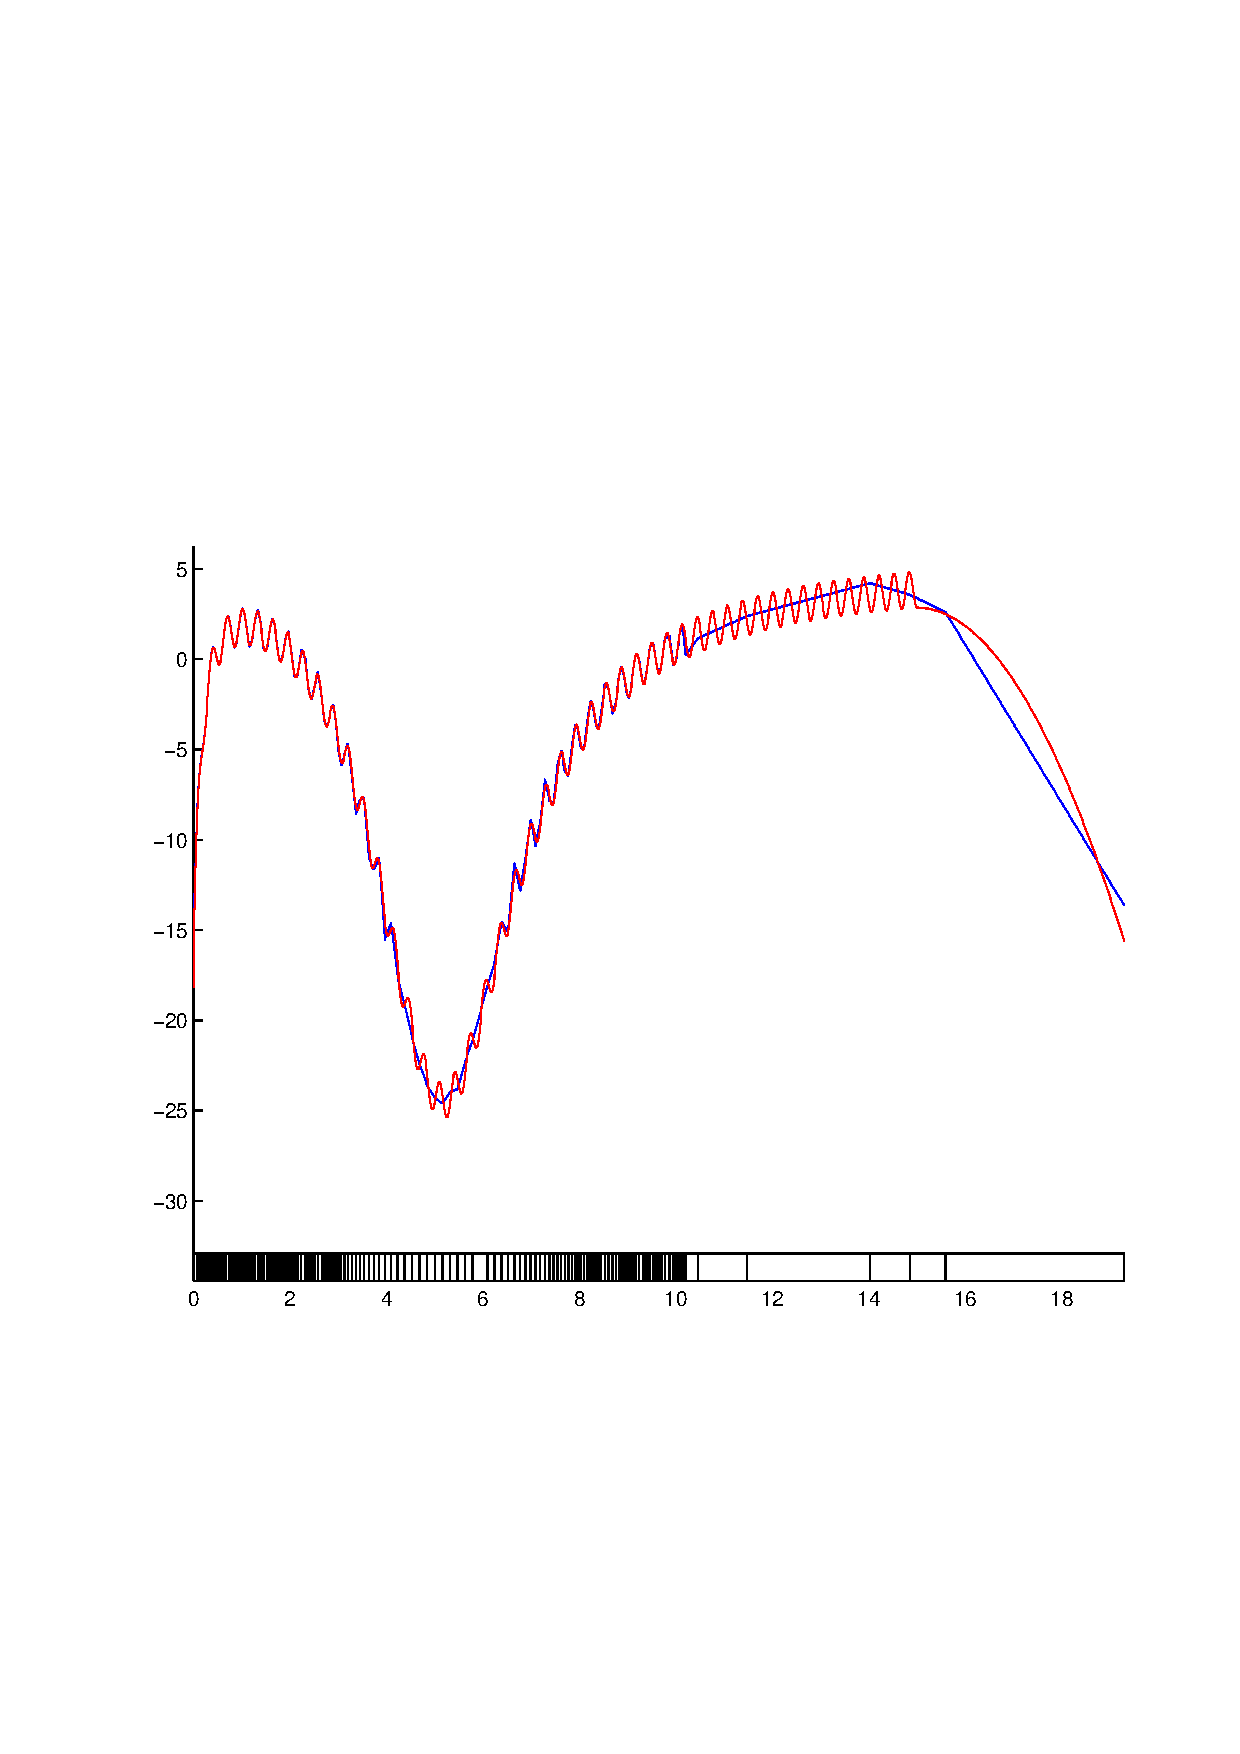
\includegraphics[width=0.3\textwidth]{Figure11} 
%\end{center}
%\caption{First preliminary numerical experiments indicating the successful recovery by an adaptive algorithm based on \eqref{fdproxy} of a potential function $a$ in a first order model of the type \eqref{fdgradientflow}. The potential $a$ to be recovered is displayed in red color and it's the strongly oscillating function. The blue function is the piecewise linear approximant computed at each successive iteration after adaptation of the underlying mesh, scketched on the bottom of the figures.}\label{firstnum}
%\end{figure}
%
%Despite the highly oscillatory nature of the parameter function $a$, the algorithm performs an excellent approximation, providing also a sort of "numerical homogenization" in those locations of the positive real line, where not enough data are provided by the evolution.

In this section we report several numerical experiments to document the validity and feasibility of Theorem \ref{thm}. We will first show how the reconstruction of a kernel gets better as the number of agents $N$ increases, in accordance with the $\Gamma$-convergence result reported in the last section. This feature holds true also for interaction kernel not lying in the function space $X$, as shown in Figure \ref{variableN2}. We will then investigate the relationship between the functional $\mathcal E_N$ and the $L_2(\R_+,\rho)$ error w.r.t. the potential $a$, and the behavior of $\mathcal E_N$ when we let the constraint $M$ vary. Finally, we will see how we can get a very satisfactory reconstruction of the unknown interaction kernel by keeping $N$ fixed and averaging the minimizers of the functional $\mathcal E_N$ obtained from several samples of the initial data distribution $\mu^0$.

\subsection{Numerical framework}\label{numfram}

All experiments will rely on a common numerical set-up, which we clarify in this section. All the initial data $\mu^N_0$ are drawn from a common probability distribution $\mu_0$ which is the uniform distribution on the $d$-dimensional cube $[-L,L]^d$. For every $\mu^N_0$, we simulate the evolution of the system starting from $\mu^N_0$ until time $T$, and we shall denote with $R$ the maximal distance between particles reached during the time frame $[0,T]$. Notice that we have at our disposal only a finite sequence of snapshots of the dynamics: if we denote with $0 = t_0 < t_1 < \ldots < t_m = T$ the time instants at which these snapshots are taken, we can consider the \textit{discrete-time error functional}
\begin{align*}
\overline{\mathcal{E}}_N(\widehat{a}) & = \frac{1}{m} \sum^m_{k = 1} \frac{1}{N} \sum^N_{j = 1} \left| \frac{1}{N} \sum^N_{i = 1} \widehat{a}(|x_j(t_k) - x_i(t_k)|)(x_j(t_k) - x_i(t_k)) - \dot{x}_i(t_k)\right|^2,
\end{align*}
which is the time-discrete counterpart of the continuous-time error functional $\mathcal{E}_N(\widehat{a})$. As already mentioned in the introduction, velocities $\dot{x}_i(t_k)$ appearing in $\overline{\mathcal{E}}_N(\widehat{a})$ are computed as finite differences, i.e.,
\begin{align*}
\dot{x}_i(t_k) = \frac{x_i(t_k) - x_i(t_{k-1})}{t_k - t_{k-1}}, \text{ for every } k \geq 1.
\end{align*}

About the reconstruction procedure, we fix the constraint $M$ and consider the sequence of invading subspaces $V_N$ generated by a linear B-spline basis with $D(N) $ elements supported on $[0,2R]$, i.e., for every element $\widehat{a} \in V_N$ it holds
\begin{align*}
	\widehat{a}(r) = \sum^{D(N)}_{\lambda = 1} a_{\lambda} \varphi_{\lambda}(r), \quad \text{for every } r \in [0,R].
\end{align*}
Since $V_N$ has to be invading, $D(N)$ is a strictly increasing function of $N$. To avoid the inconvenience of having a reconstructed kernel with value at $0$ and at $R$ equal to $0$, we consider the knots of the B-spline basis to be
\begin{align}\label{eq:knots}
\left[0,0,0,\frac{R}{(D(N)-2)},\ldots,\frac{(D(N) - 3)R}{(D(N)-2)},R,R,R\right],
\end{align}
i.e., the spline reconstruction has in $0$ and $R$ two discontinuity points.

Whenever $\widehat{a} \in V_N$, we can rewrite the functional $\mathcal{E}_N(\widehat{a})$ as
\begin{align*}
\overline{\mathcal{E}}_N(\widehat{a}) & = \frac{1}{m} \sum^m_{k = 1} \frac{1}{N} \sum^N_{j = 1} \left| \frac{1}{N} \sum^N_{i = 1} \sum^{D(N)}_{\lambda = 1} a_{\lambda} \varphi_{\lambda}(|x_j(t_k) - x_i(t_k)|)(x_j(t_k) - x_i(t_k)) - \dot{x}_i(t_k)\right|^2 \\
& = \frac{1}{m} \sum^m_{k = 1} \frac{1}{N} \sum^N_{j = 1} \left| \sum^{D(N)}_{\lambda = 1} a_{\lambda} \frac{1}{N} \sum^N_{i = 1} \varphi_{\lambda}(|x_j(t_k) - x_i(t_k)|)(x_j(t_k) - x_i(t_k)) - \dot{x}_i(t_k)\right|^2 \\
& = \frac{1}{mN} \left\| C \vec{a} - v \right\|^2_{2},
\end{align*}
where $\vec{a} = (a_1, \ldots, a_{D(N)})$, $v = (\dot{x}_1(t_1), \ldots, \dot{x}_N(t_1), \ldots,\dot{x}_1(t_m), \ldots, \dot{x}_N(t_m))$ and $C \in \R^{d\times Nm \times D(N)}$ satisfies for every $j = 1, \ldots,N$, $k = 1, \ldots,m$, $\lambda = 1, \ldots,D(N)$
\begin{align*}
C(jk,\lambda) = \frac{1}{N} \sum^N_{i = 1} \varphi_{\lambda}(|x_j(t_k) - x_i(t_k)|)(x_j(t_k) - x_i(t_k)) \in \R^d.
\end{align*}

We shall numerically implement the constrained minimization with the software CVX, which allows constraints and objectives to be specified using standard MATLAB expression syntax. In order to use it, we need to rewrite the constraint of our minimization problem, which reads
\begin{align*}
	\|a\|_{L_{\infty}([0,R])} + \|a'\|_{L_{\infty}([0,R])} \leq M,
\end{align*}
using only the minimization variable of the problem, which is the vector of coefficients of the B-spline basis $\vec{a}$. Notice that the property of being a linear B-spline basis implies that, for every $\lambda = 1, \ldots, D(N)-1$, the property $\supp(\varphi_{\lambda}) \cap \supp(\varphi_{\lambda + j}) \not= \emptyset$ holds if and only if $j = 1$. Hence, for every $a \in V_N$ we have
\begin{align*}
\|a\|_{L_{\infty}([0,R])} &= \max_{r \in [0,R]} \left|\sum^{D(N)}_{\lambda = 1} a_{\lambda} \varphi_{\lambda}(r)\right|
% \leq \max_{r \in [0,R]} \sum^{D(N)}_{\lambda = 1} \left|a_{\lambda} \varphi_{\lambda}(r)\right| 
 \leq \max_{\lambda = 1, \ldots, D(N)-1} \left(|a_{\lambda}| + |a_{\lambda+1}|\right) 
 \leq 2 \|\vec{a}\|_{\infty},
\end{align*}
\begin{align*}
\|a'\|_{L_{\infty}([0,R])} &= \max_{r \in [0,R]} \left|\sum^{D(N)}_{\lambda = 1} a_{\lambda} \varphi'_{\lambda}(r)\right| 
 \leq \max_{\lambda = 1, \ldots, D(N)-1} |a_{\lambda+1} - a_{\lambda}|
 = \|D\vec{a}\|_{\infty},
\end{align*}
where, in the last line, $D$ is the matrix
\begin{align*}
D = \begin{bmatrix}
    1       & -1 & 0 & \dots & 0 & 0 \\
    0     & 1 & -1 & \dots & 0 & 0 \\
   \vdots & \vdots & \ddots & \ddots & \vdots & \vdots \\ \\
    0       & 0 & 0 & \dots & 1 & -1 \\
    0       & 0 & 0 & \dots & 0 & 0
\end{bmatrix}.
\end{align*}
We numerically implement the constrained minimization problem
\begin{align*}
\min_{\widehat{a} \in V_N} \mathcal{E}_N(\widehat{a}) \quad \text{ subject to } \quad \|\widehat{a}\|_{L_{\infty}([0,R])} + \|\widehat{a}'\|_{L_{\infty}([0,R])} \leq M,
\end{align*}
in the following way
\begin{align}\label{problem2}
\min_{\vec{a} \in \R^{D(N)}} \frac{1}{mN} \left\| C \vec{a} - v \right\|^2_{2} \quad \text{ subject to } \quad 2\|\vec{a}\|_{\infty} + \|D\vec{a}\|_{\infty} \leq M.
\end{align}
The byproduct of the time discretization and the reformulation of the constraint is that minimizers of problem \eqref{problem2} may not be minimizers of the original one. This is the price to pay for the numerical implementation of the theoretical result. However, we will see how in practice the modifications we made are so mild that we obtain very satisfactory reconstructions of the unknown potential, and moreover we still observe the approximation properties proved in the previous sections.

\subsection{Varying $N$}

In Figure \ref{variableN} we show the reconstruction of a truncated Lennard-Jones type interaction kernel obtained with different values of $N$. The following table reports the values of the different problem's parameters.

\begin{table}[h]
\begin{center}
\begin{tabular}{ |c|c|c|c|c|c| }
\hline
  $d$ & $L$ & $T$ & $M$ & $N$ & $D(N)$ \\
\hline
\hline
  $2$ & $3$ & $0.5$ & $100$ & $[10,20,40,80]$ & $2N$ \\
\hline
\end{tabular}
\end{center}
\vspace{-0.5cm}
\caption{Parameter values for Figure \ref{variableN} and Figure \ref{variableN2}} \label{tab:fig1} 
\end{table}

It is clearly visible how the the piecewise linear approximant (displayed in blue) gets closer and closer to the potential to be recovered (in red), as predicted by the theoretical results of the previous sections. What is however surprising is that the same behavior is witnessed in Figure \ref{variableN2}, where the algorithm is applied to an interaction kernel $a$ not belonging to the function space $X$ (due to its singularity at the origin) with the same specifications reported in Table \ref{tab:fig1}. The algorithm performs an excellent approximation despite the highly oscillatory nature of the function $a$.

\begin{figure}[h!]
\begin{center}
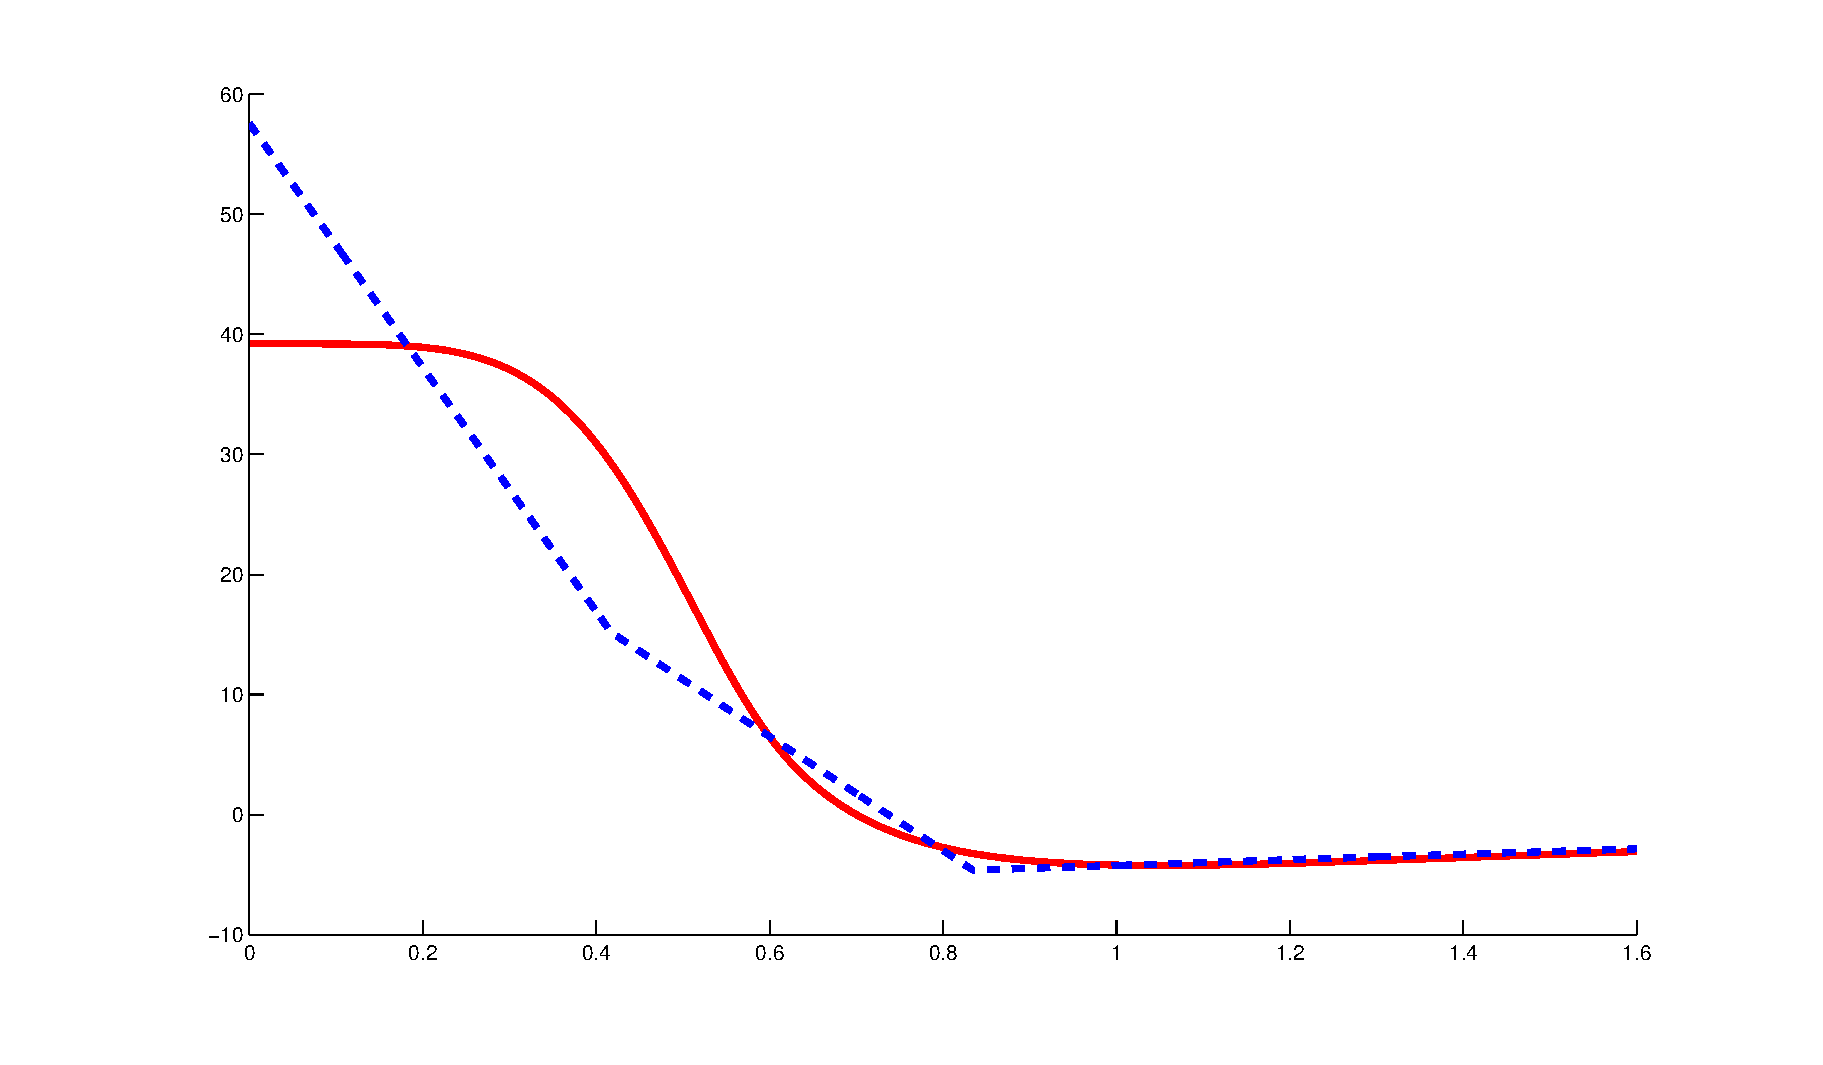
\includegraphics[width=0.45\textwidth]{figfun810agents}
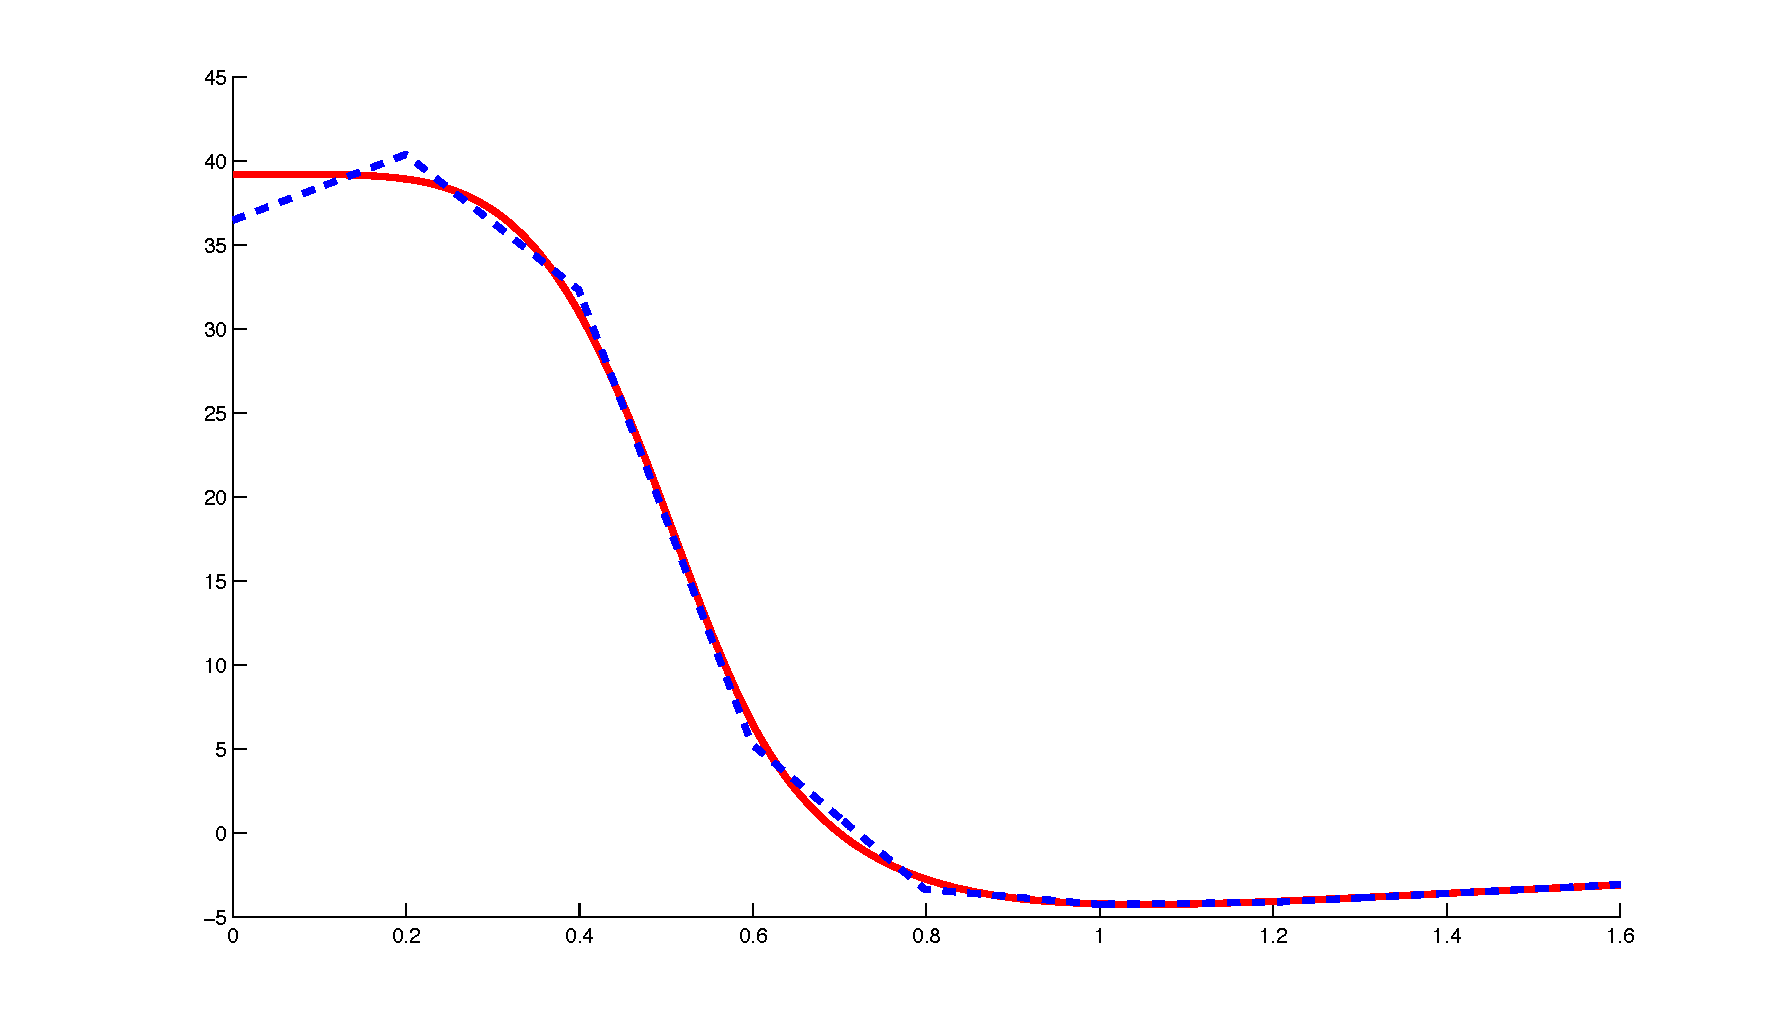
\includegraphics[width=0.45\textwidth]{figfun820agents}\\
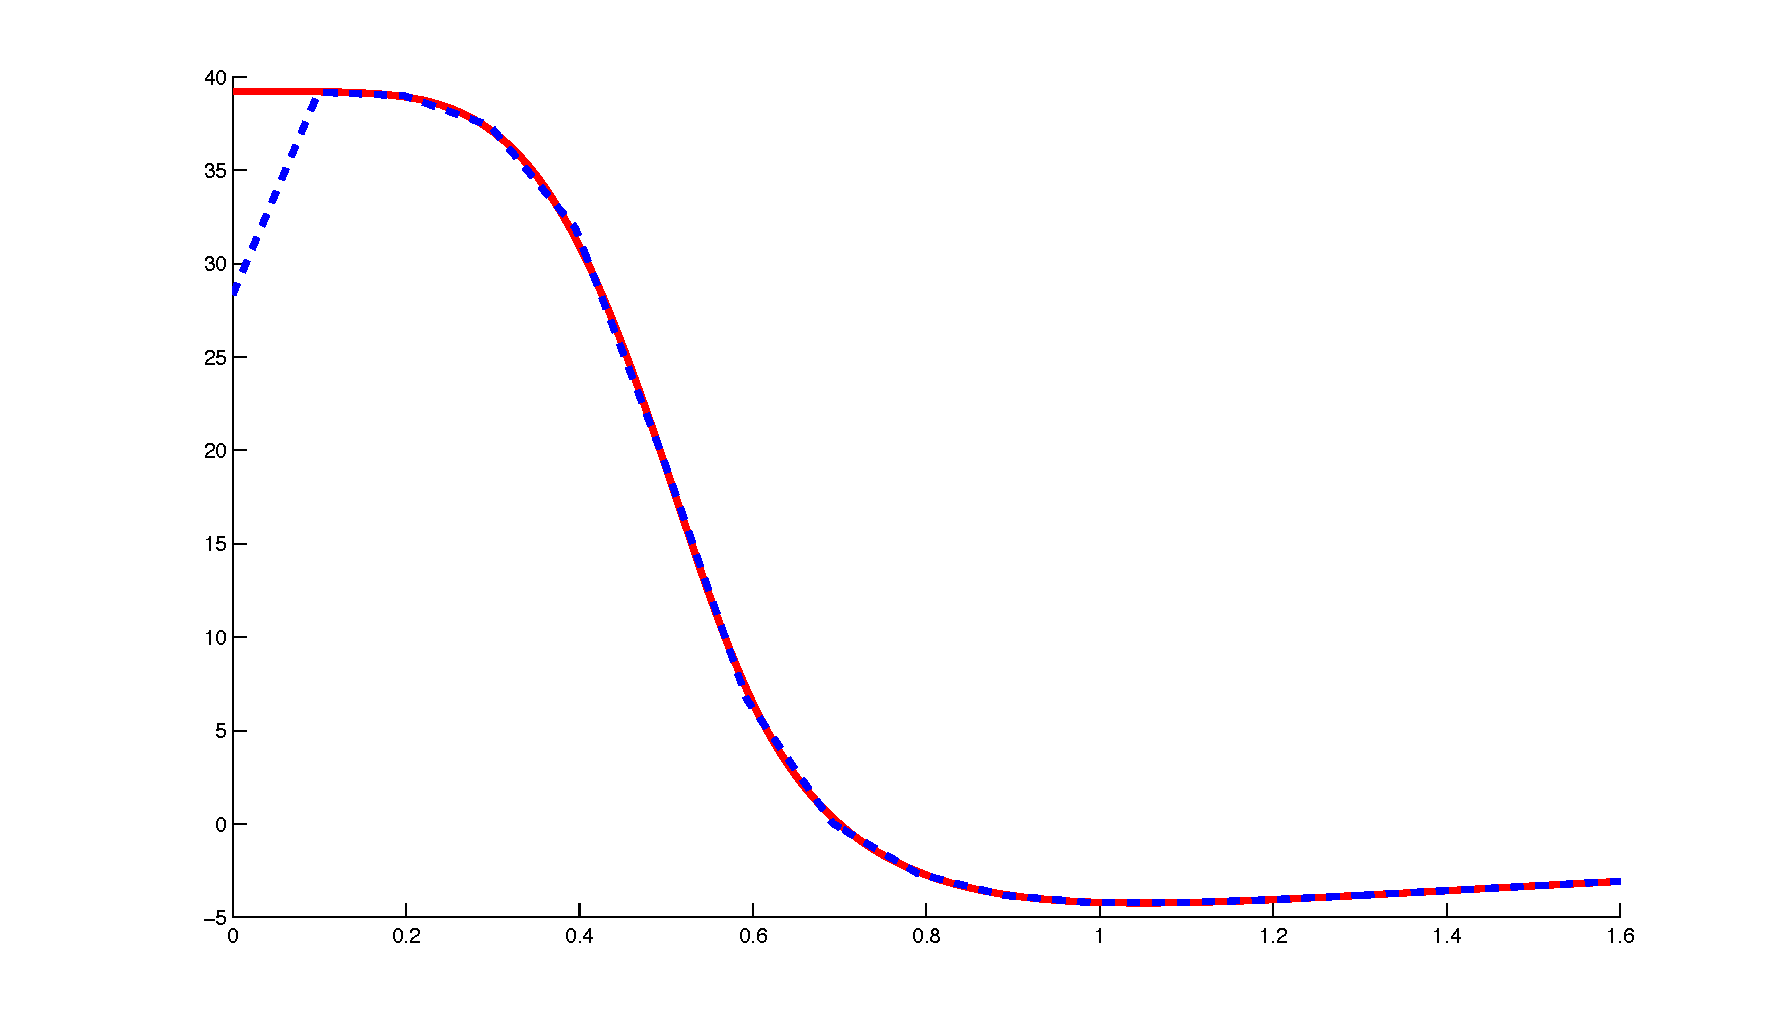
\includegraphics[width=0.45\textwidth]{figfun840agents}
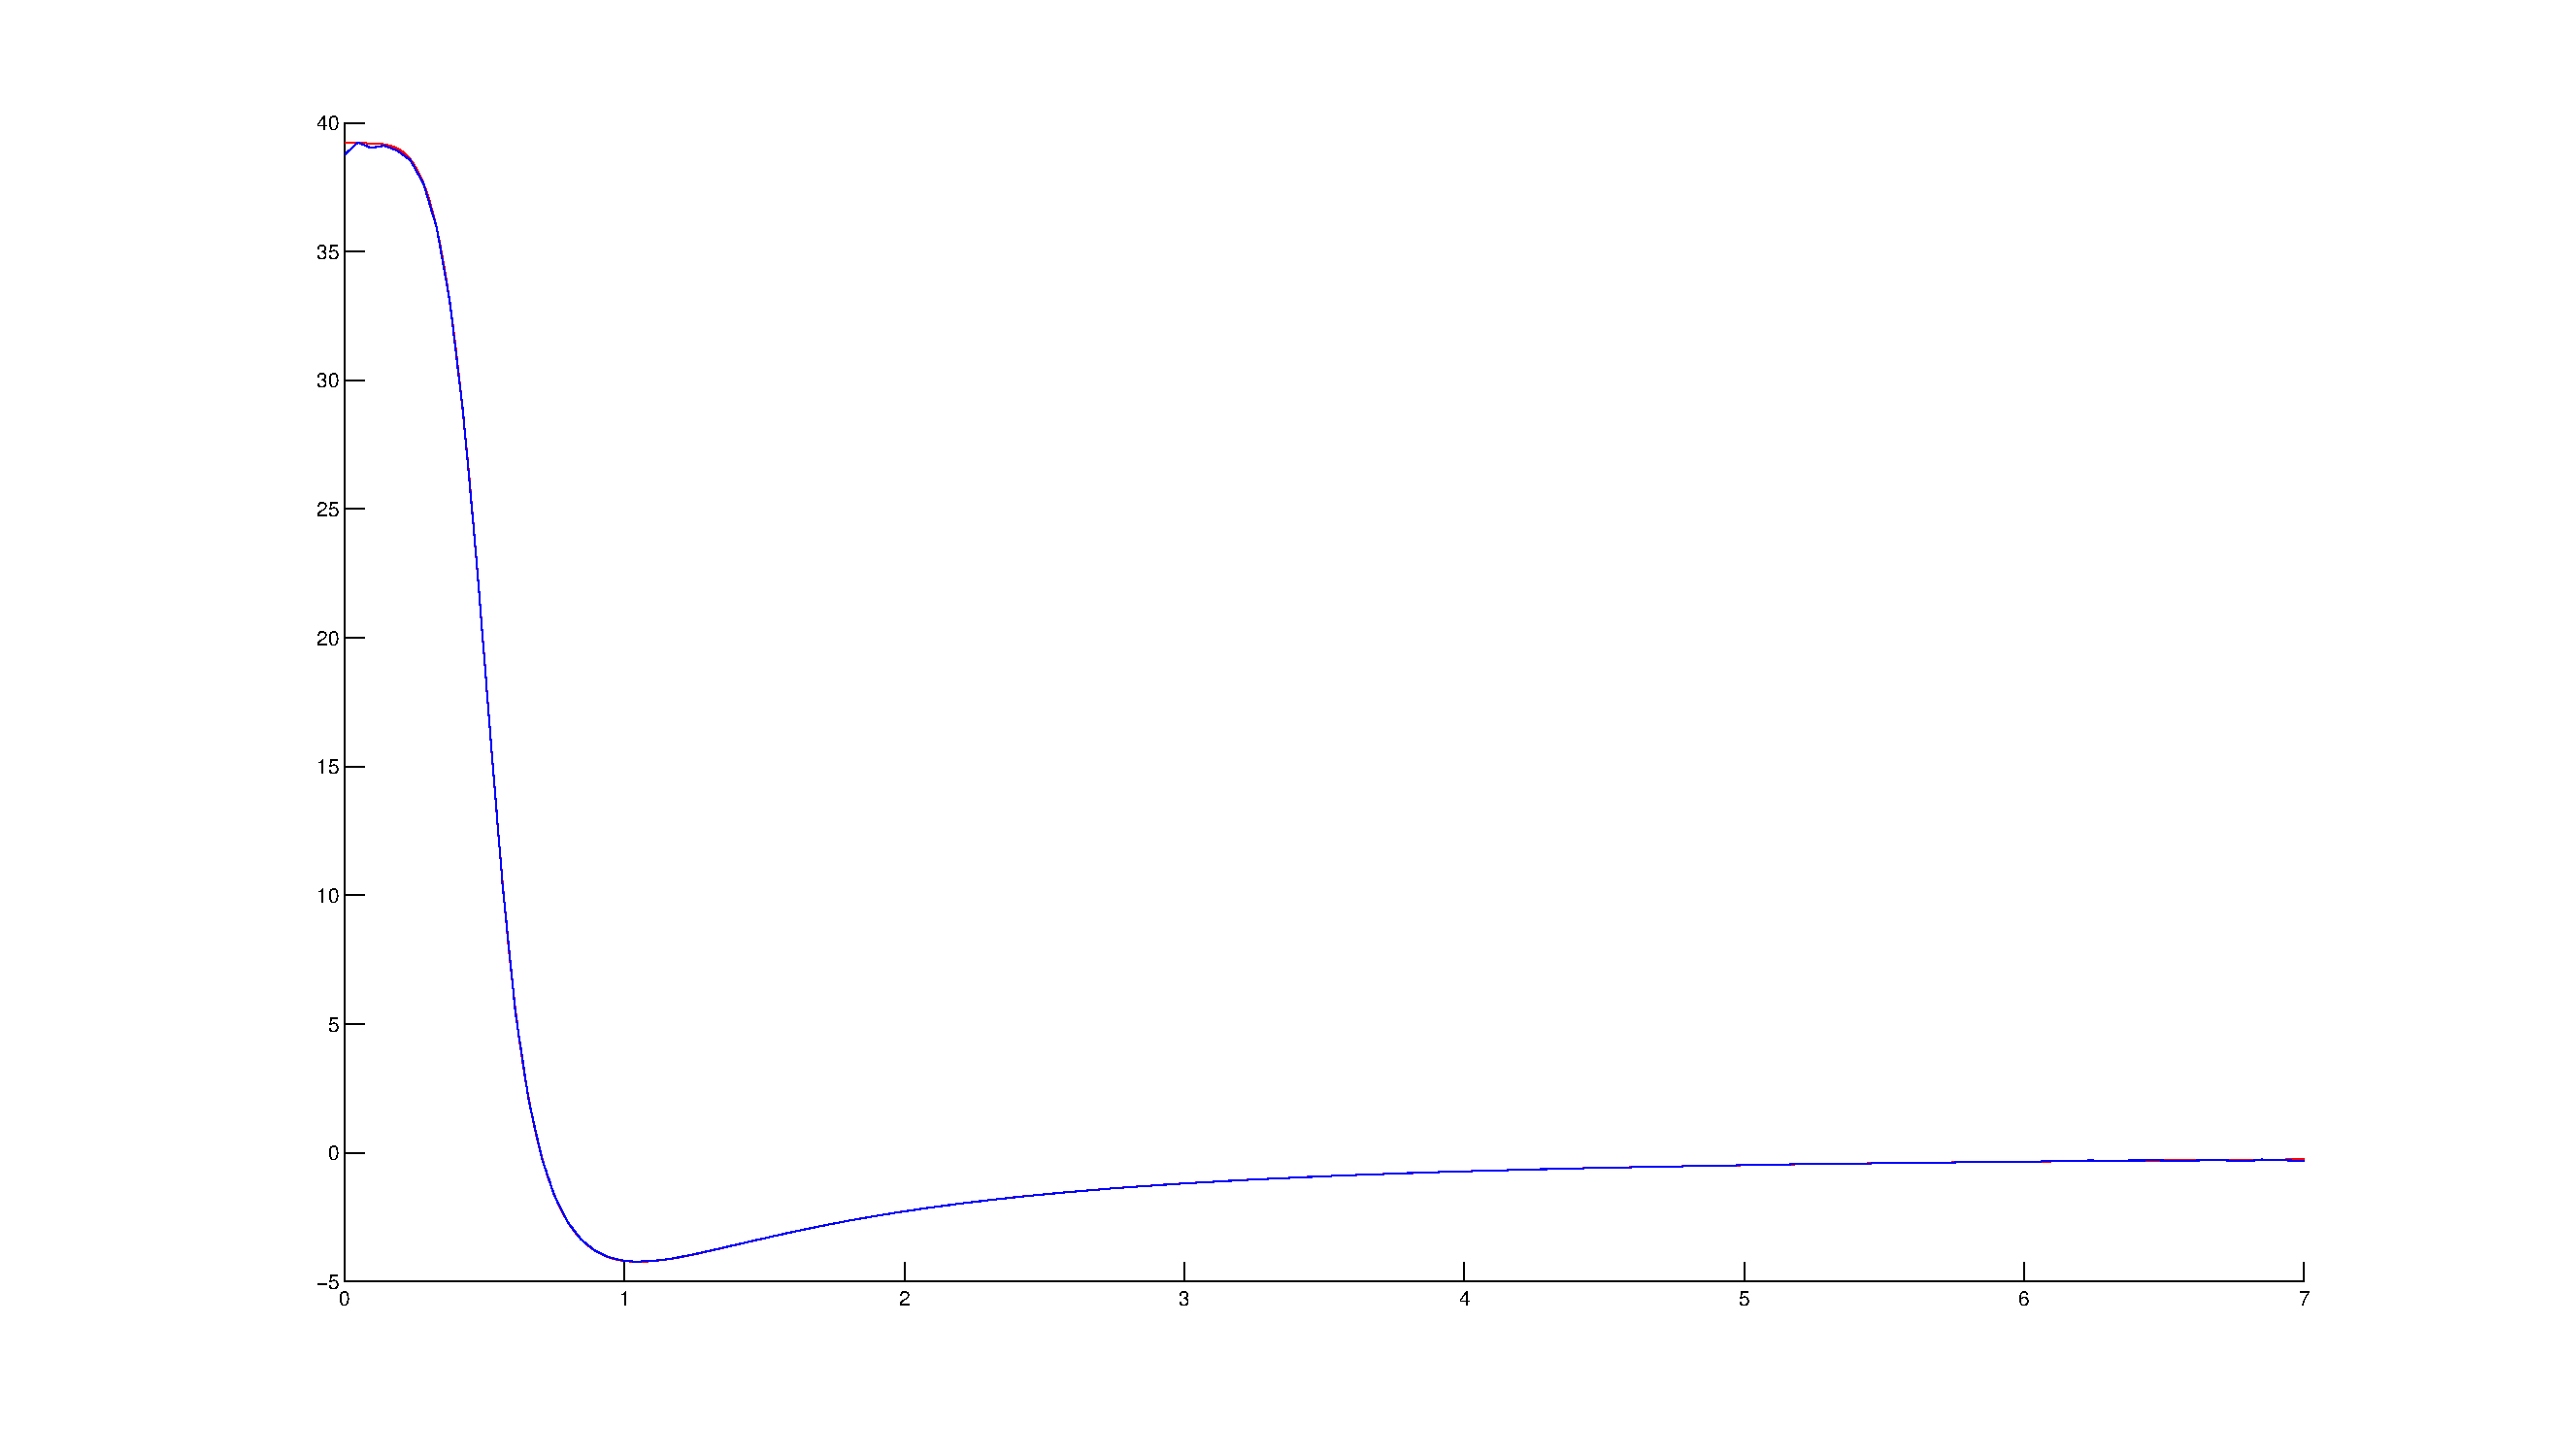
\includegraphics[width=0.45\textwidth]{figfun880agents}
\end{center}
\caption{Iterative reconstruction of a potential with different values of $N$. In red: the unknown kernel. In blue: its reconstruction by minimization of $\mathcal{E}_N$. From left-top to right-bottom: reconstruction with $N = 10$, $N = 20$, $N = 40$, $N = 80$ agents.}\label{variableN}
\end{figure}

\begin{figure}[h!]
\begin{center}
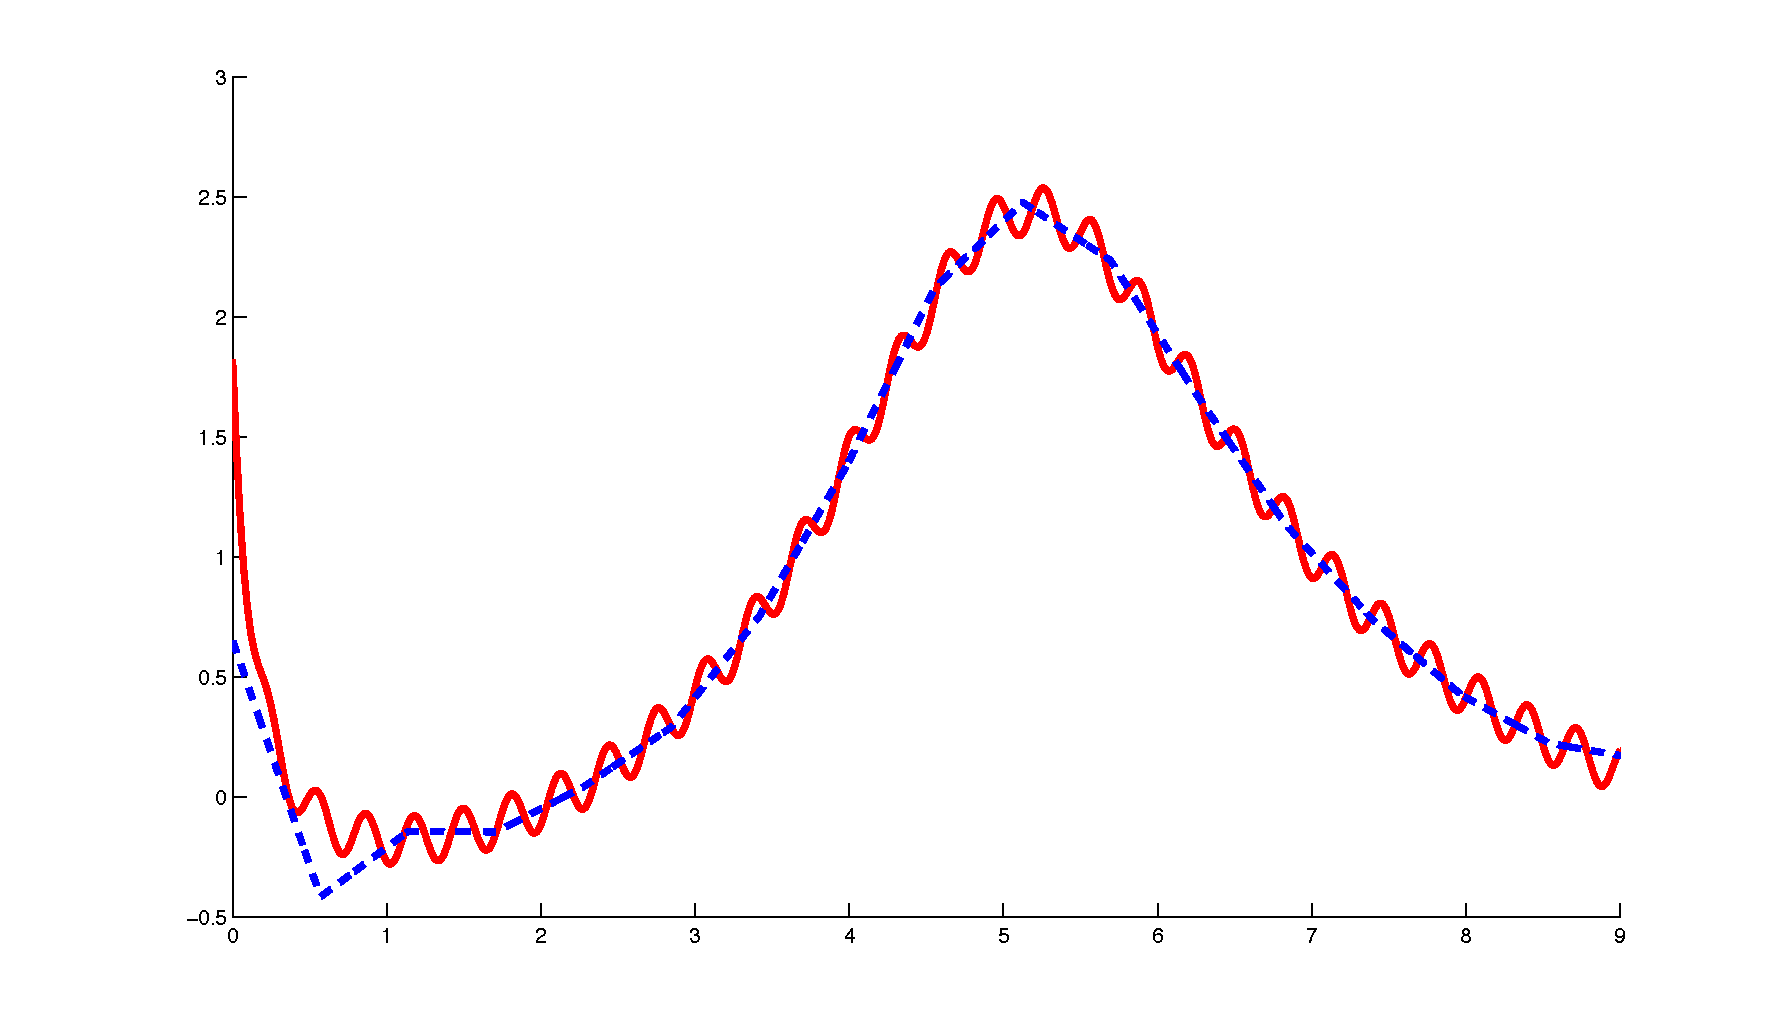
\includegraphics[width=0.45\textwidth]{figfun610agents}
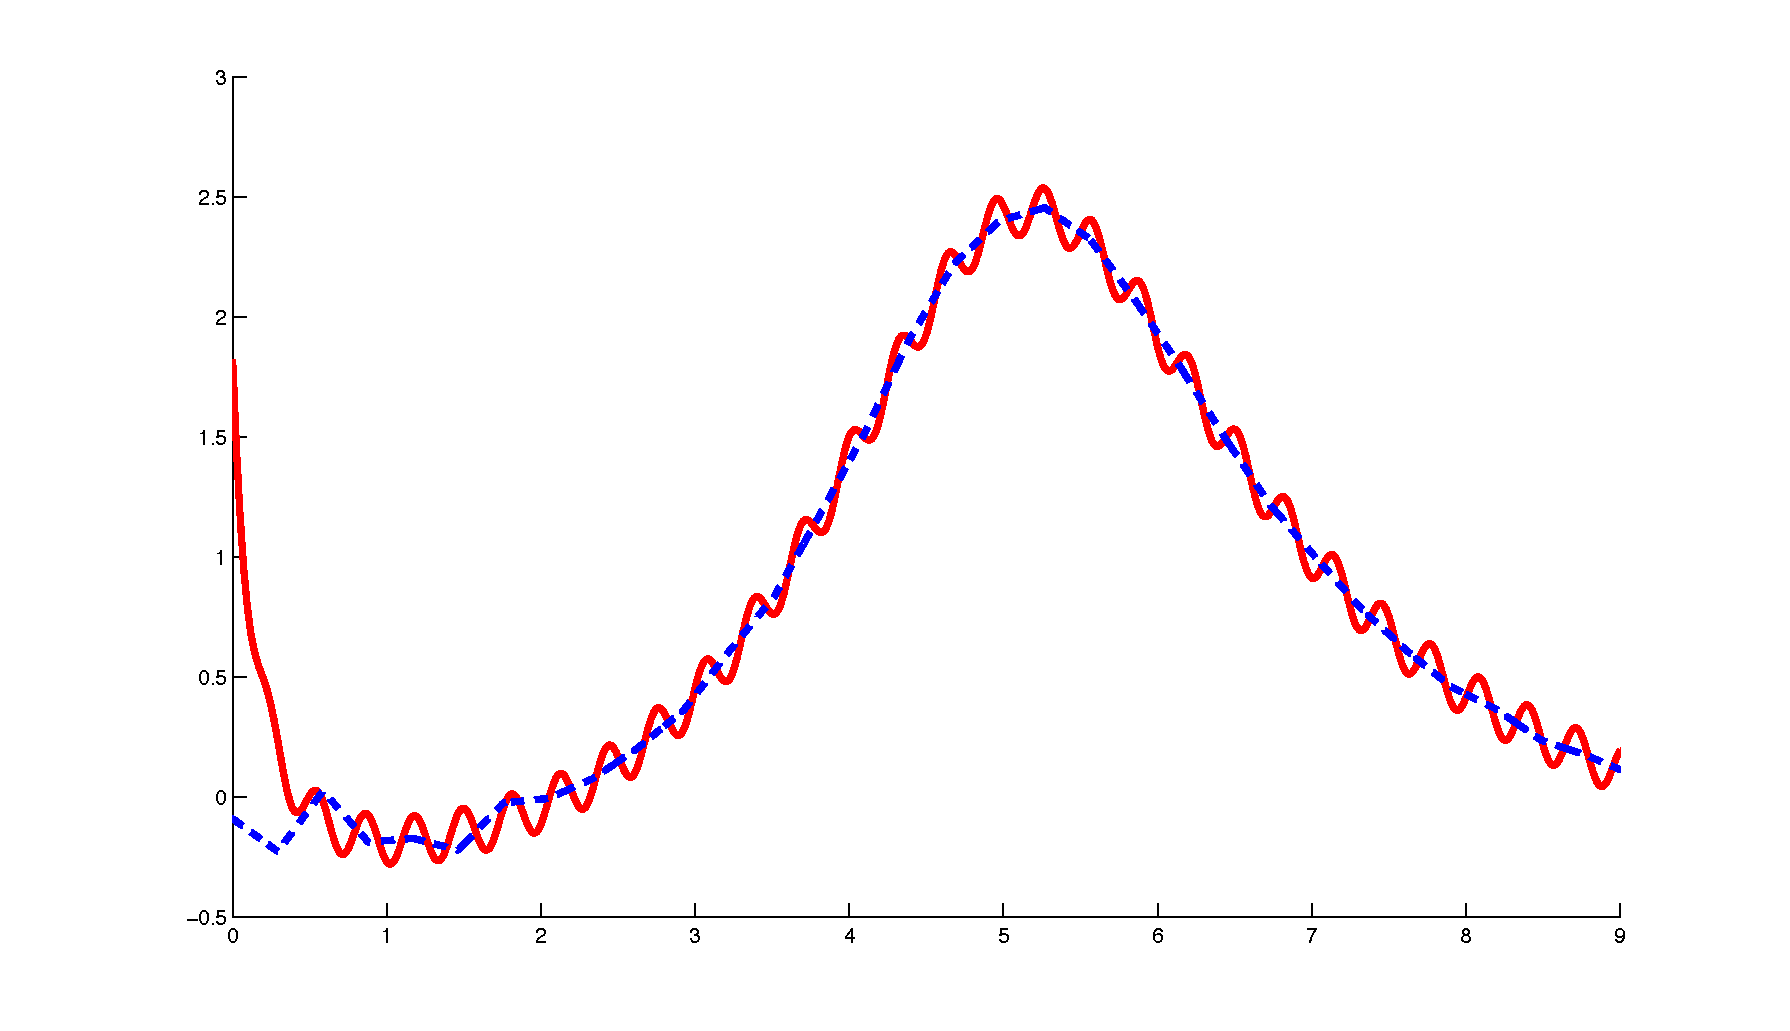
\includegraphics[width=0.45\textwidth]{figfun620agents}\\
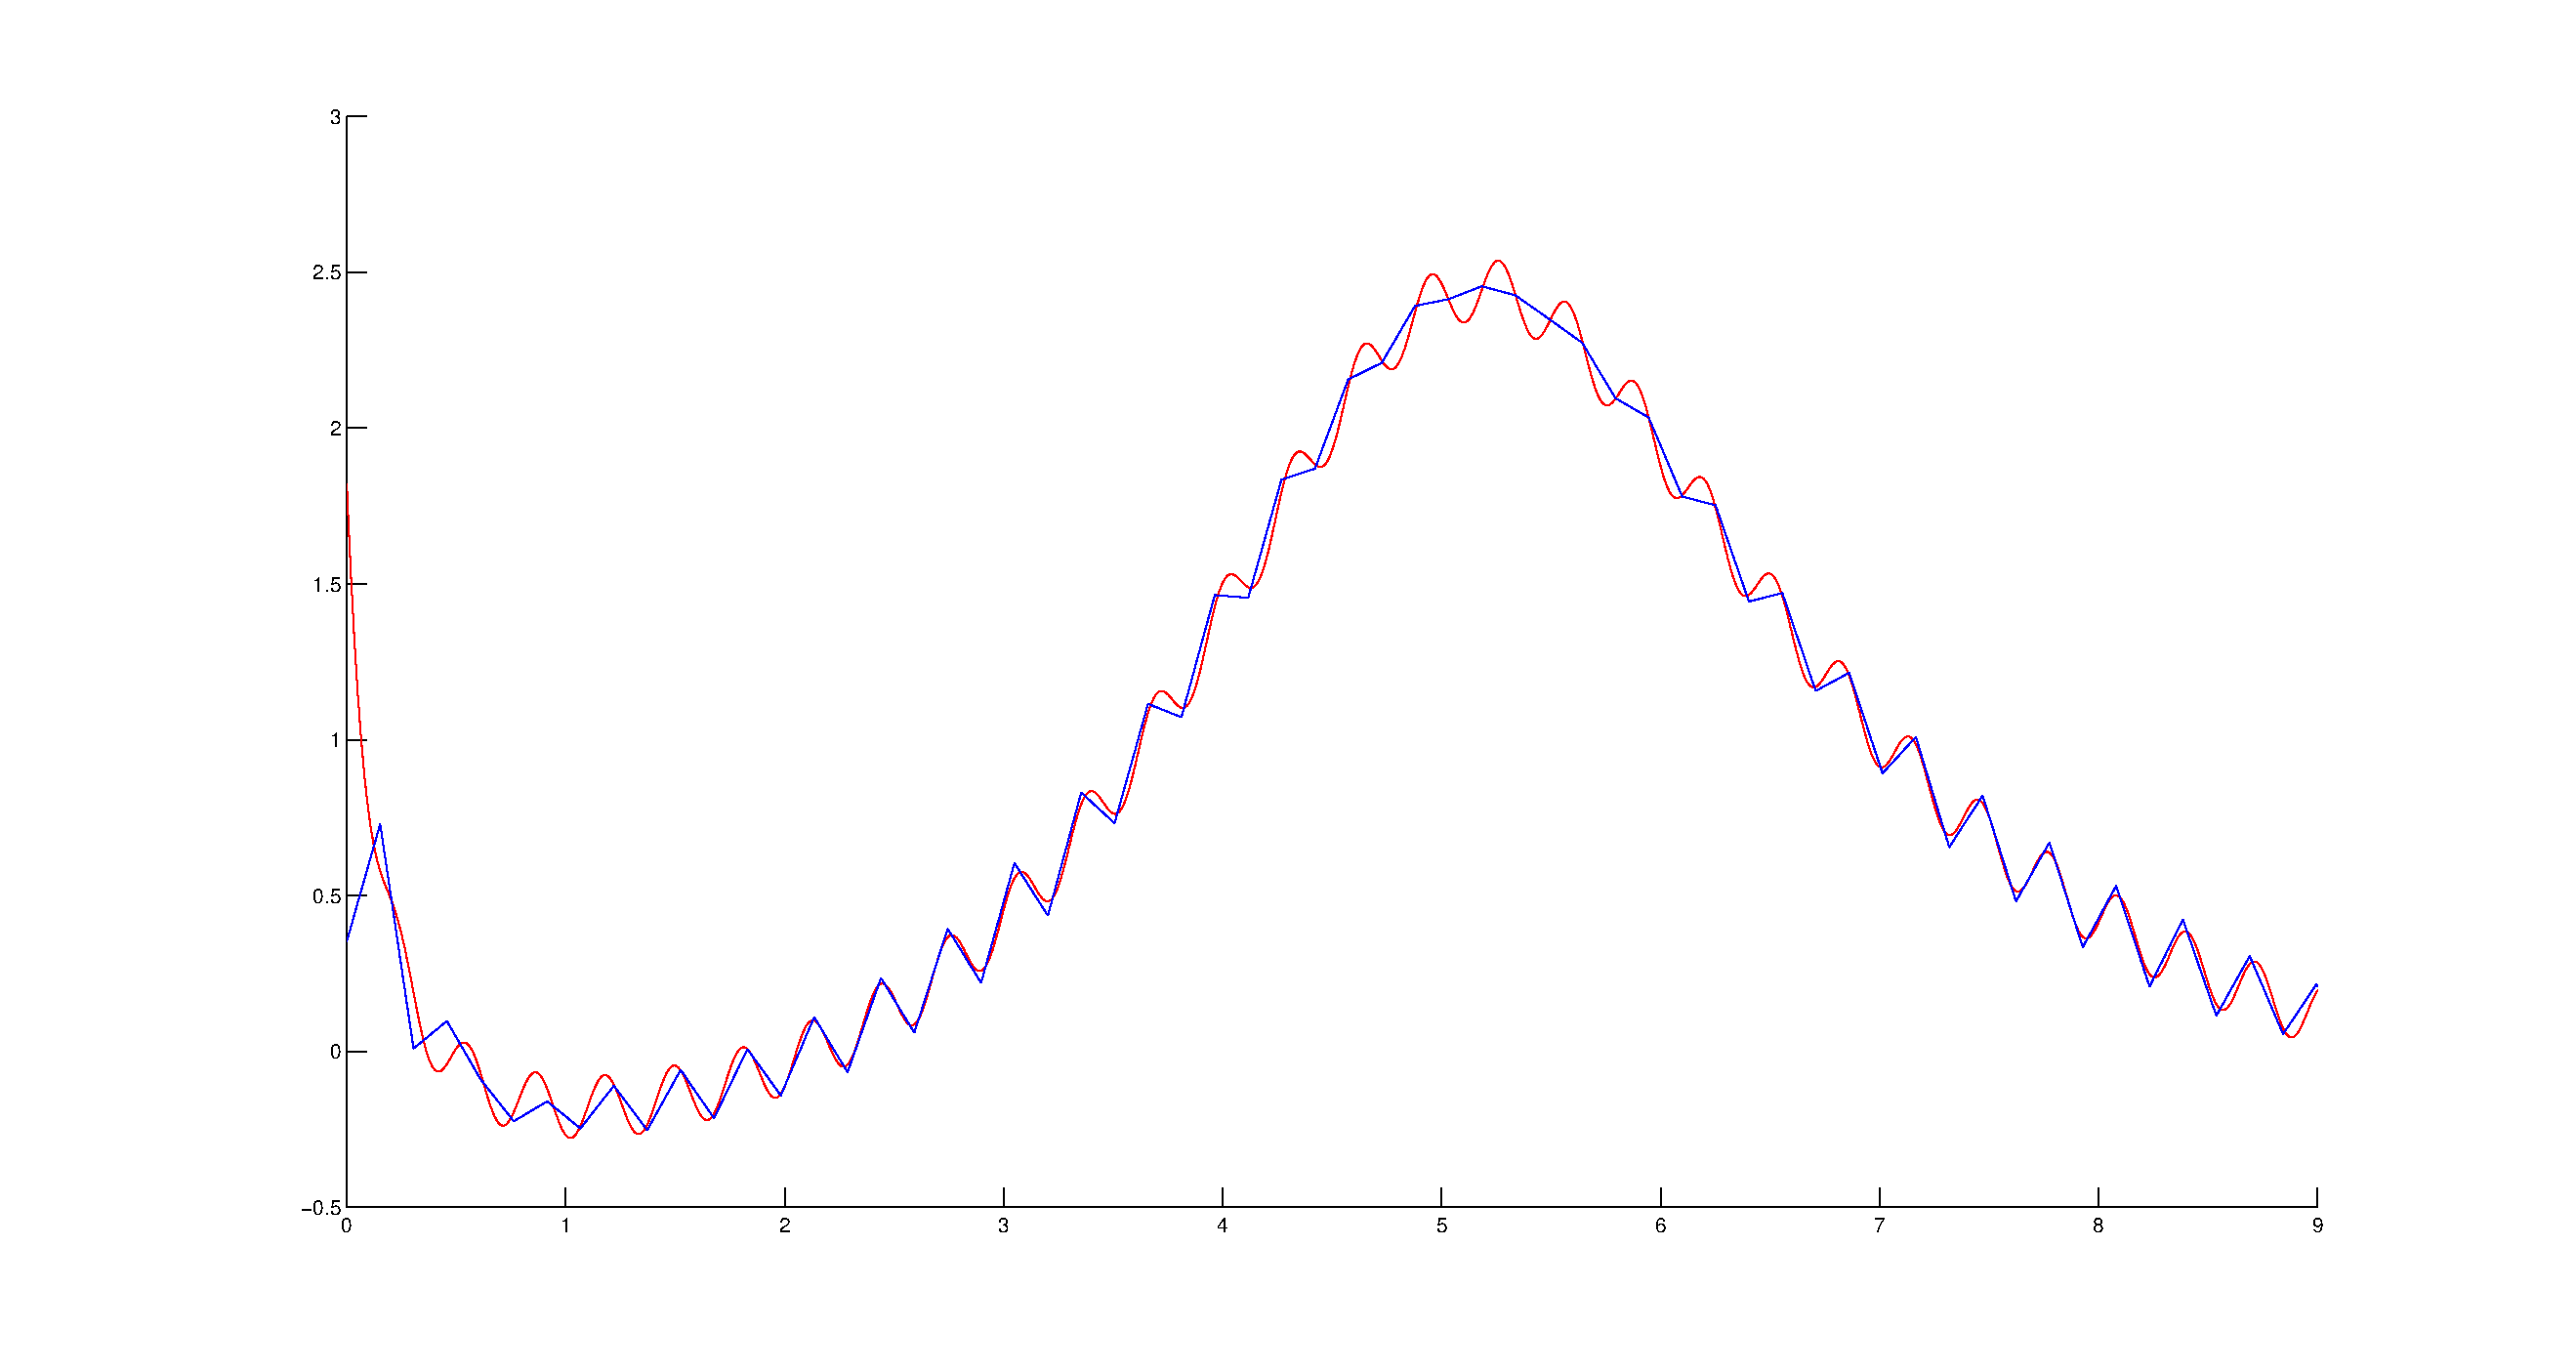
\includegraphics[width=0.45\textwidth]{figfun640agents}
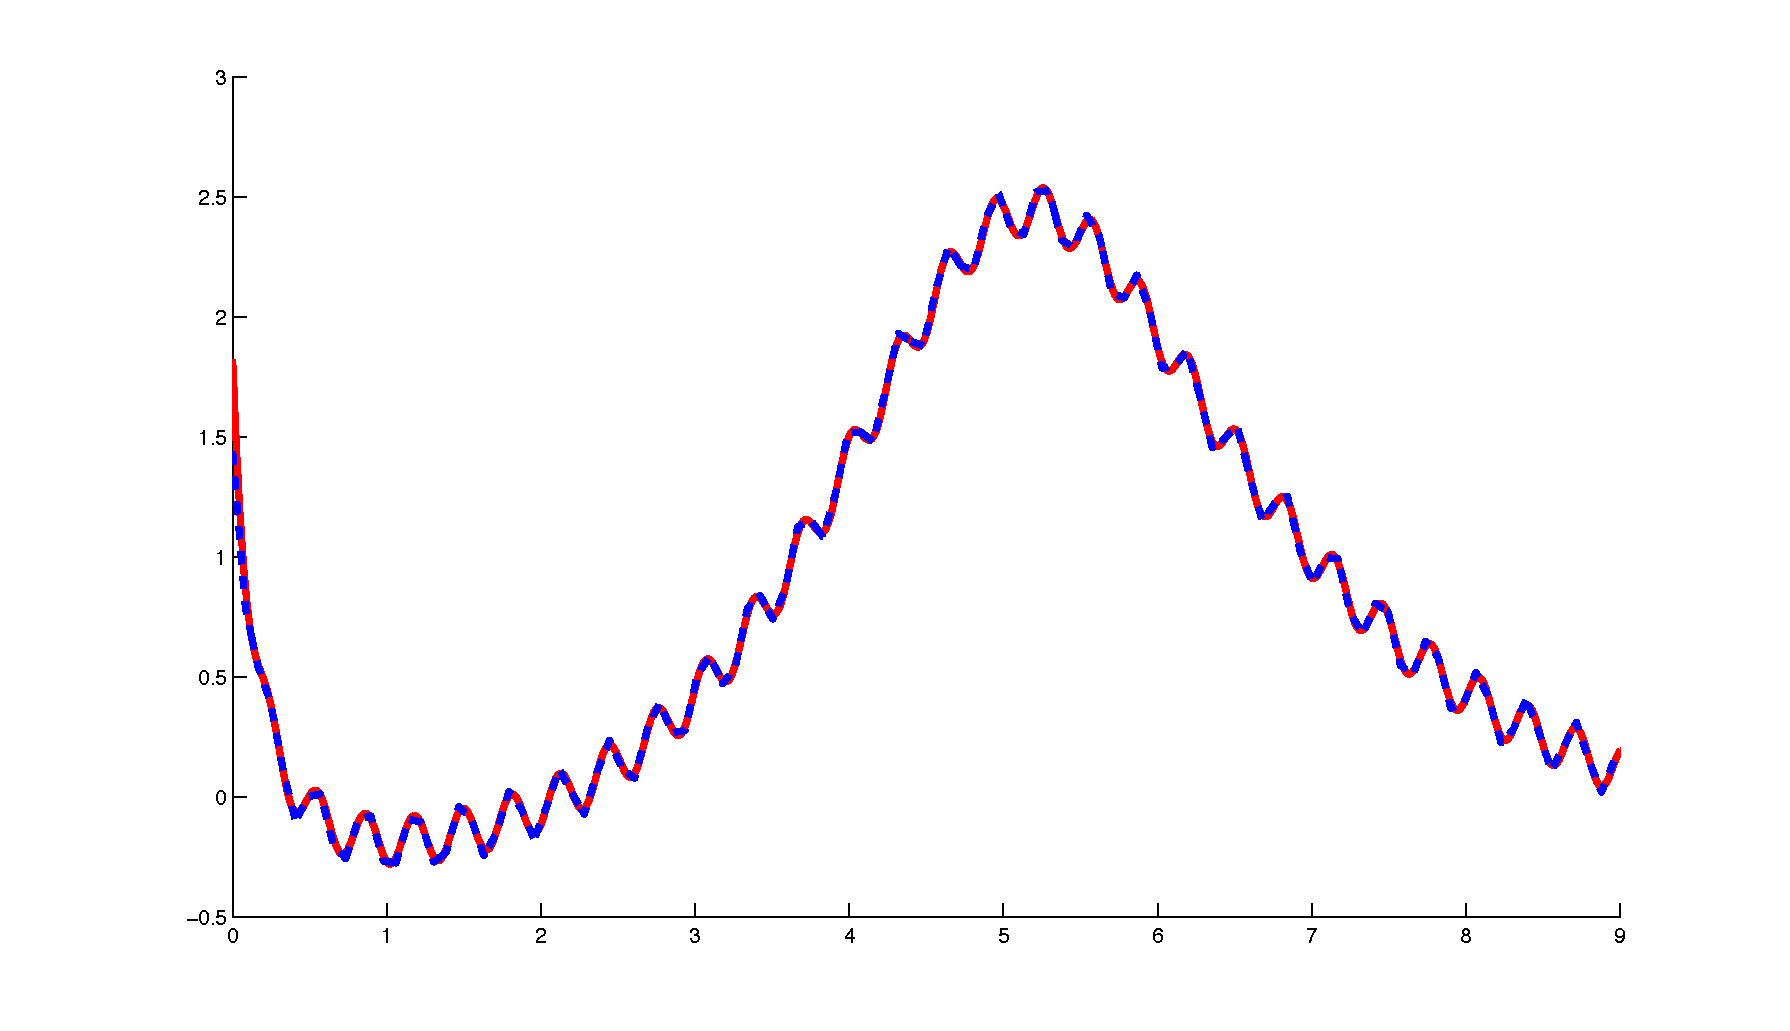
\includegraphics[width=0.45\textwidth]{figfun680agents}
\end{center}
\caption{Iterative reconstruction of a potential with a singularity at the origin and highly oscillatory behavior. In red: the unknown kernel. In blue: its reconstruction by minimization of $\mathcal{E}_N$. From left-top to right-bottom: reconstruction with $N = 10$, $N = 20$, $N = 40$, $N = 80$ agents.}\label{variableN2}
\end{figure}

\subsection{The coercivity constant}

We now turn our attention to the coercivity constant $c_T$ appearing in \eqref{eq-coercive} and thoroughly discussed in Section \ref{sec:coerc}. In Figure \ref{errorN} we see a comparison between the evolution of the value of the error functional $\overline{\mathcal{E}}_N(\widehat{a}_N)$ and of the $L_2(\R_+,\rho)$-error $\|a-\widehat{a}_N\|^2_{L_2(\R_+,\rho)}$ for different values of $N$. 

\begin{figure}[h]
\hspace{-1.2cm}
\begin{minipage}{0.58\textwidth}
\begin{center}
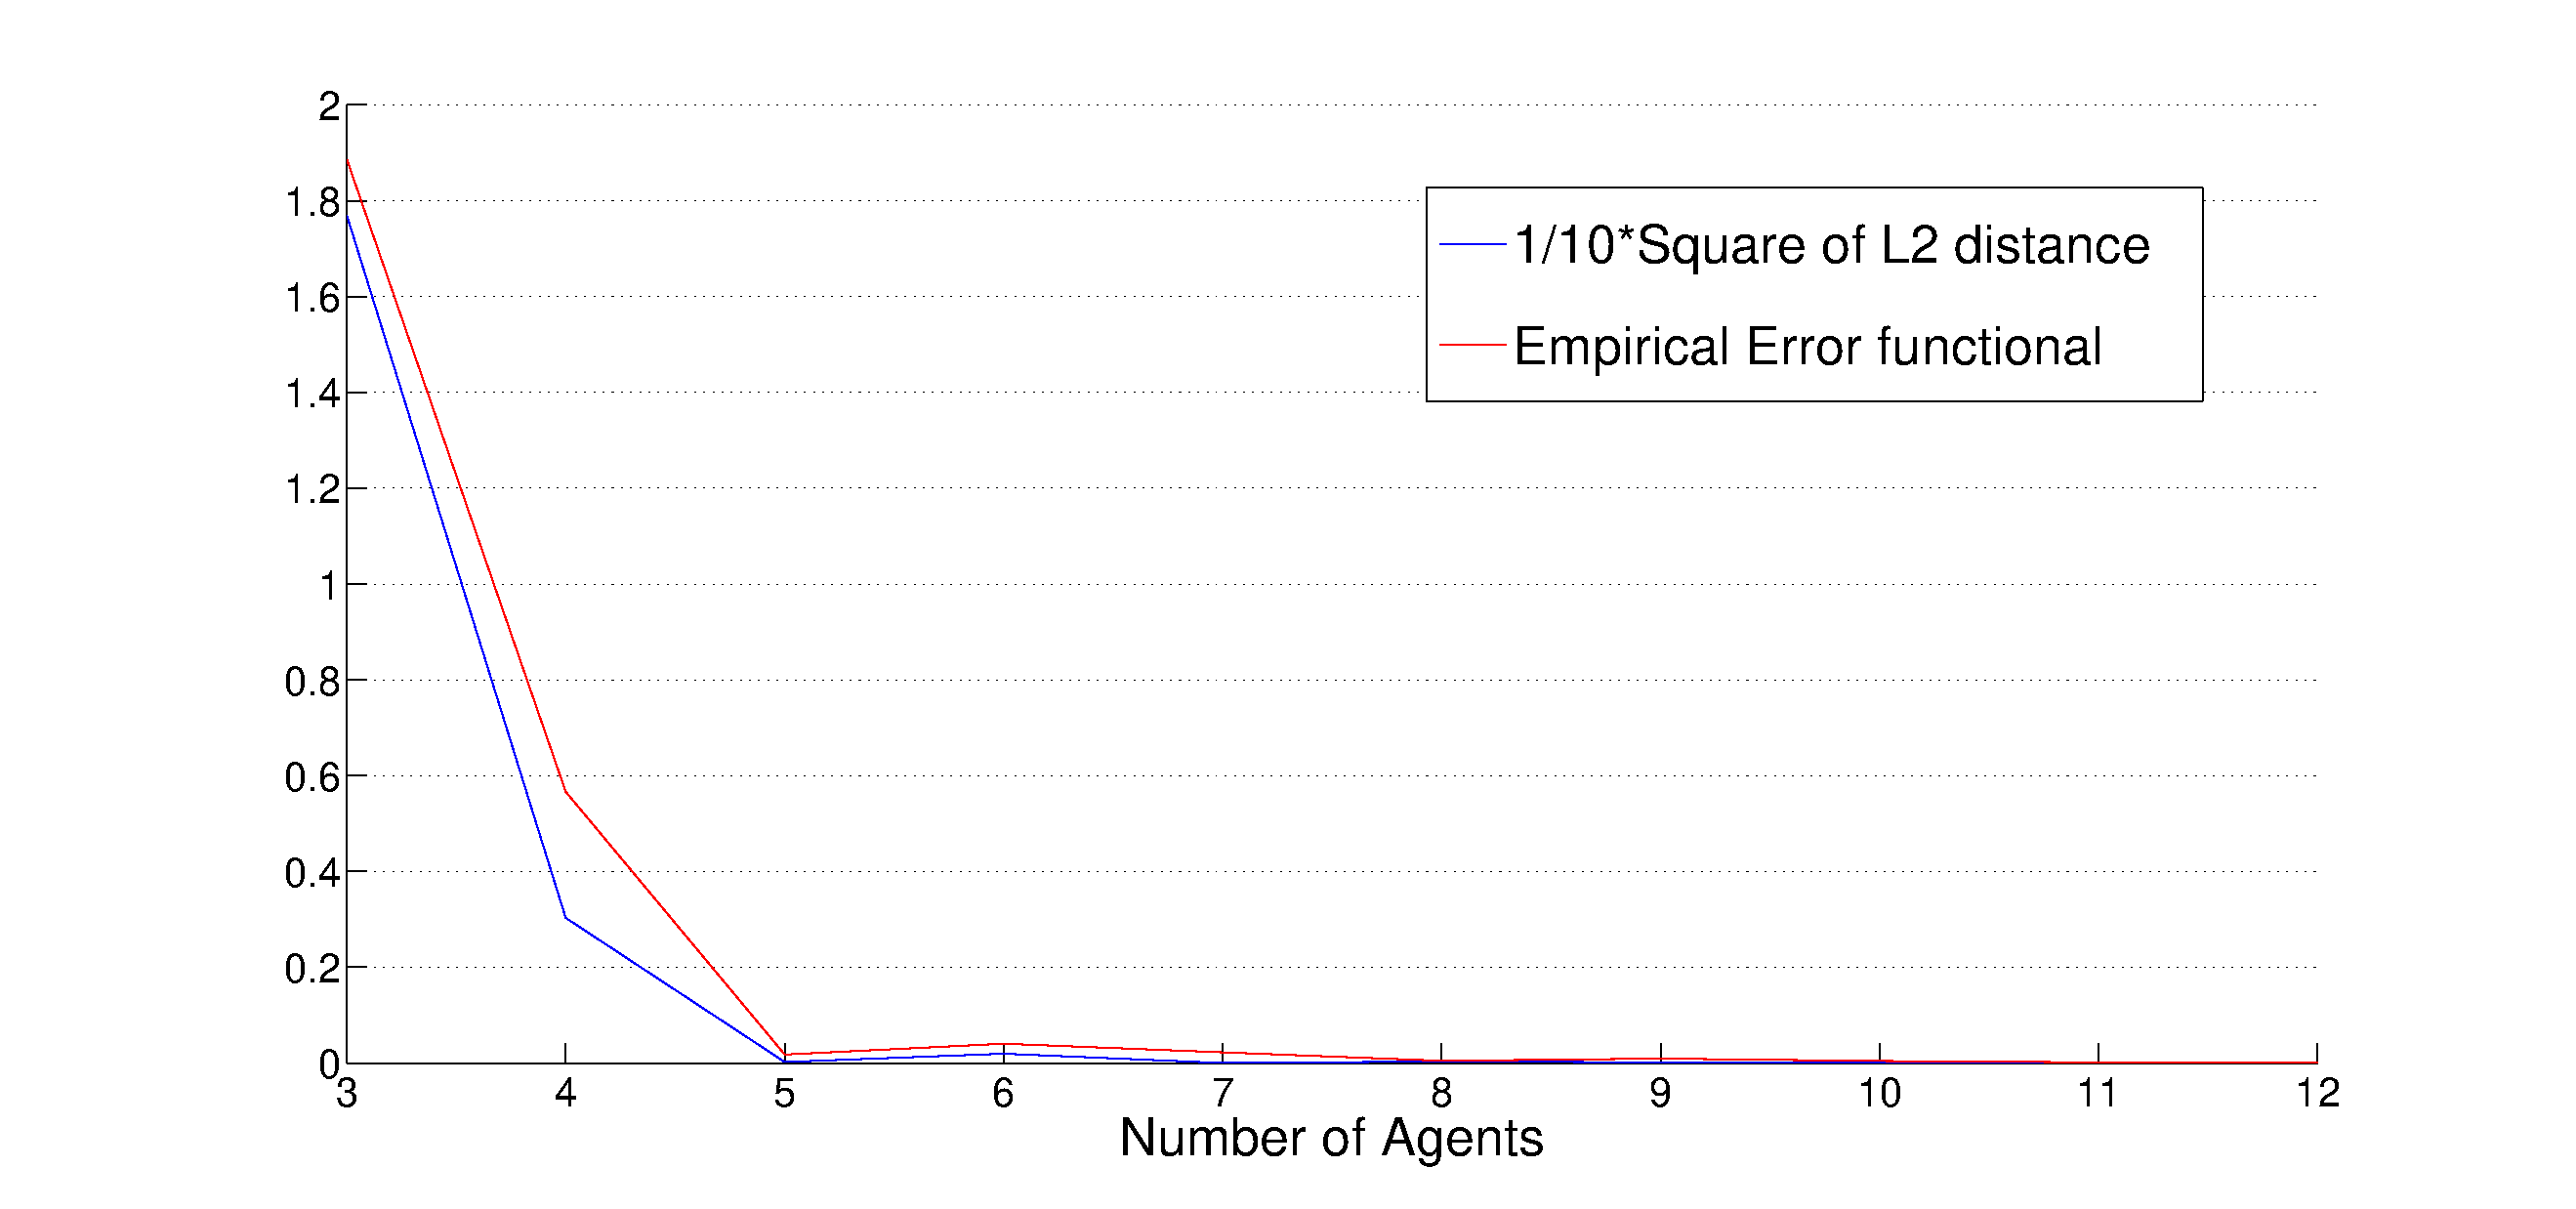
\includegraphics[width=1\textwidth]{figErrorN.eps}
\end{center}
\caption{Plot of $\overline{\mathcal{E}}_N(\widehat{a}_N)$ and $\frac{1}{10}\|a-\widehat{a}_N\|^2_{L_2(\R_+,\rho)}$ for different values of $N$. In this experiment, we can estimate the constant $c_T$ with the value $\frac{1}{10}$. \MMcomment{I would make this a $\log$ plot, i.e. with teh $y$-axis in $\log_{10}$ (or $\log_2$) scale}}\label{errorN}
\end{minipage}
\hspace{0.4cm}
\begin{minipage}{0.55\textwidth}
\begin{center}
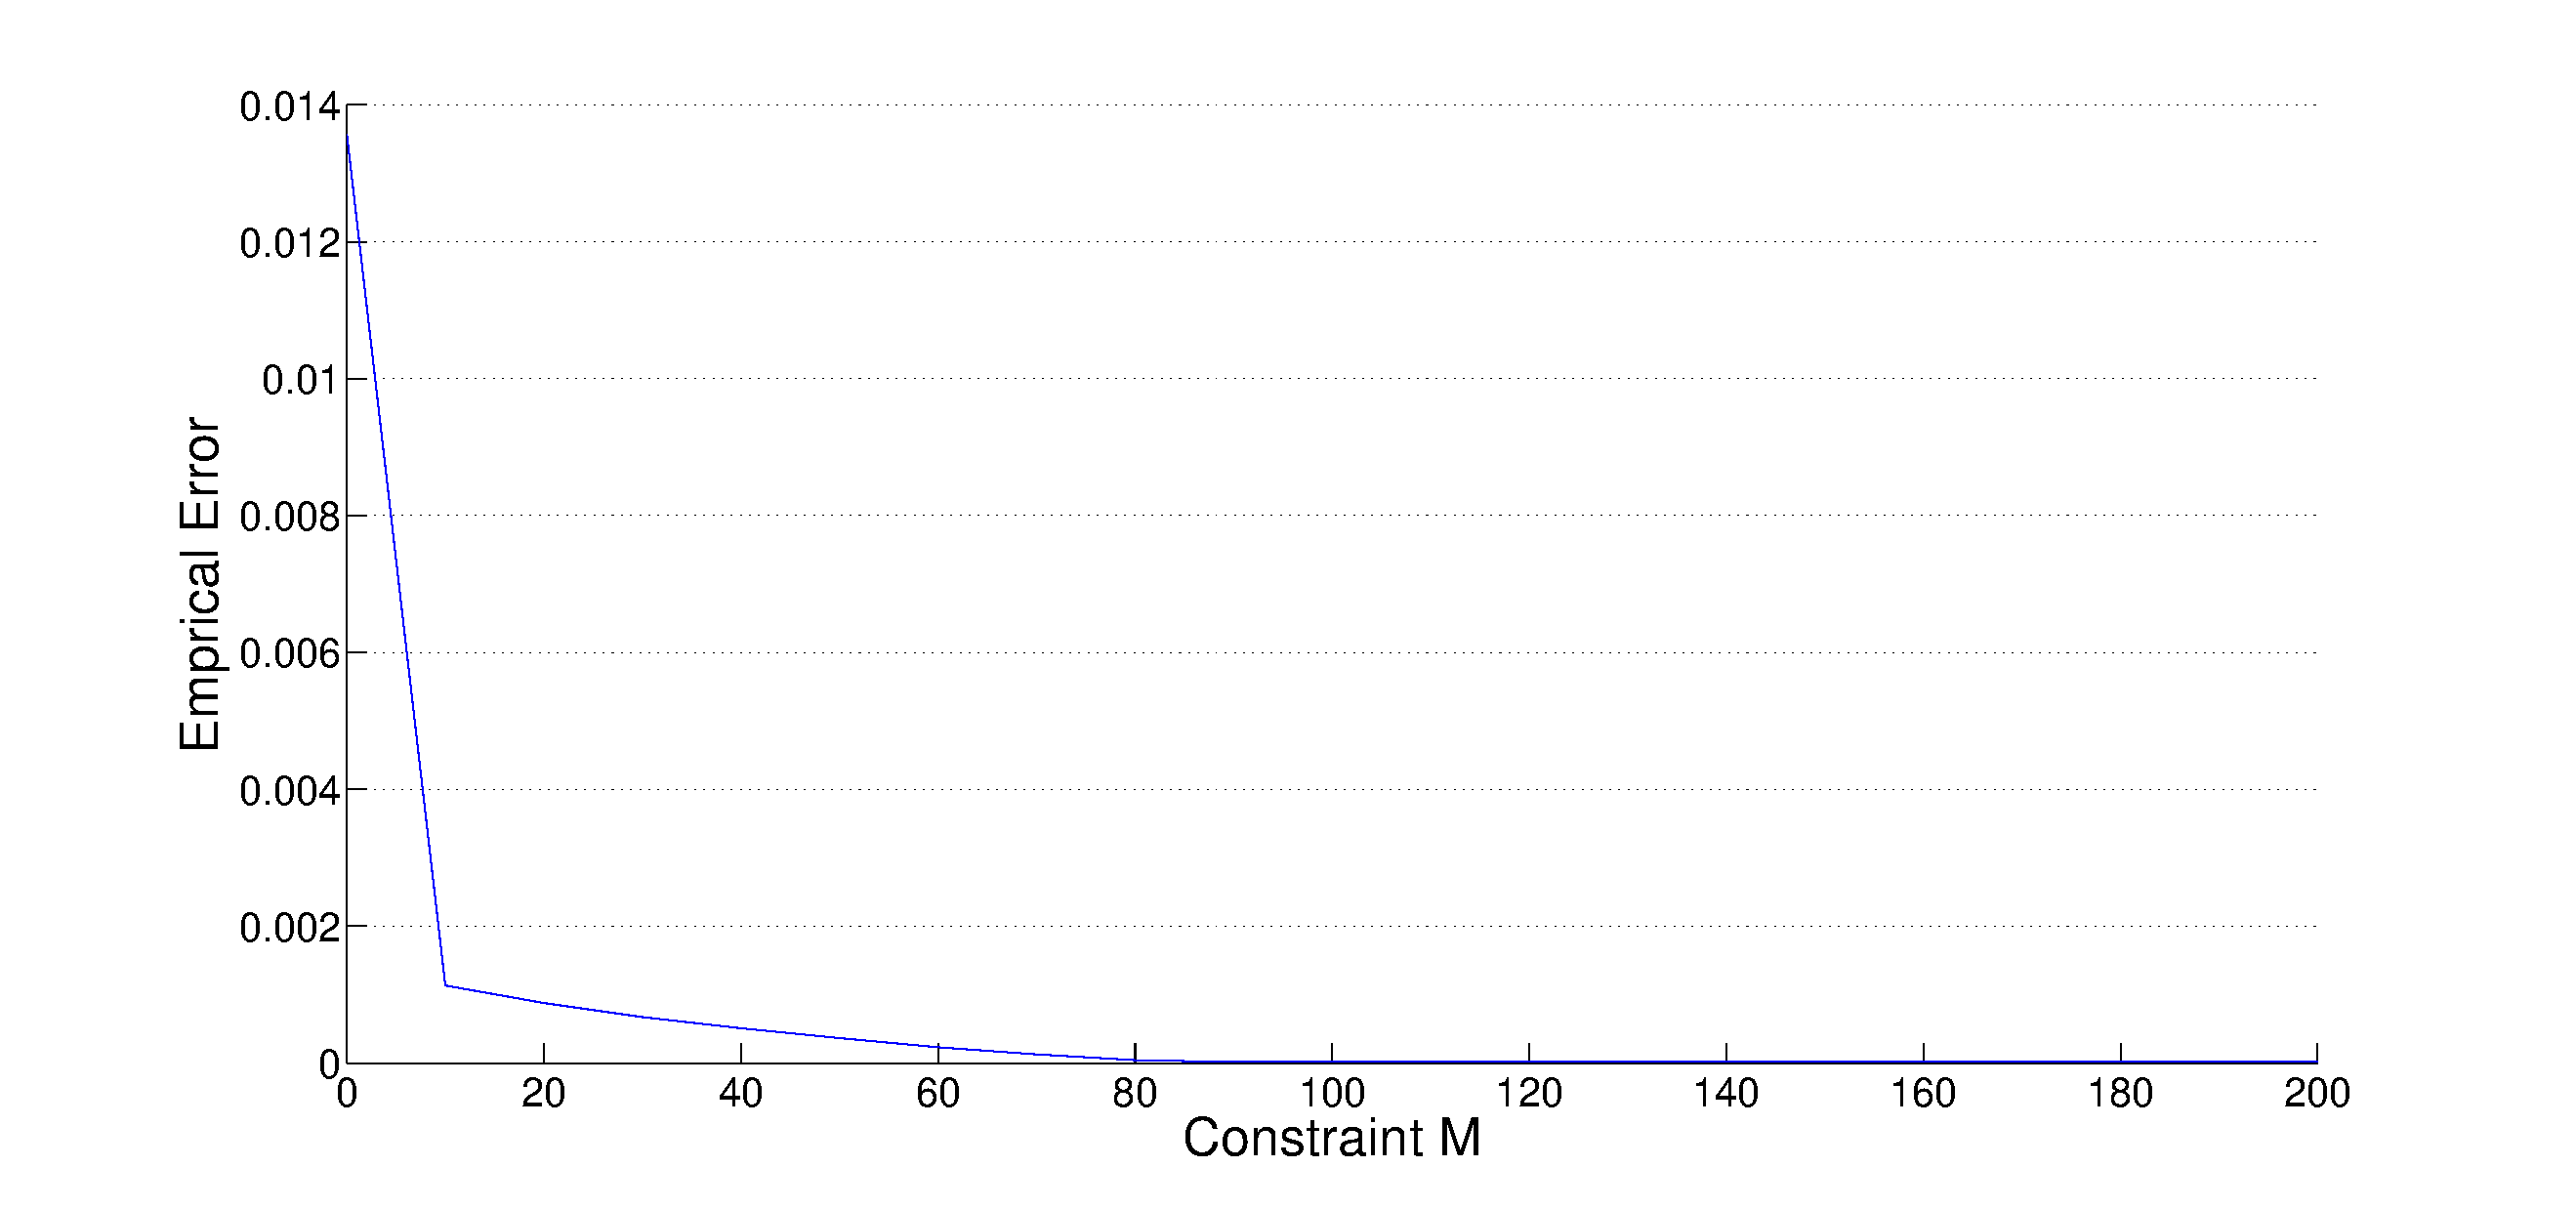
\includegraphics[width=1\textwidth]{figM.eps}
\end{center}
\caption{Values of $\overline{\mathcal{E}}_N$ for fixed $N = 50$ for different values of $M \in [0,200]$.\MMcomment{I would make this a $\log$ plot, i.e. with teh $y$-axis in $\log_{10}$ (or $\log_2$) scale}}\label{Mconstr}
\end{minipage}
\end{figure}

In this experiment, the potential $a$ to be retrieved is the truncated Lennard-Jones type interaction kernel of Figure \ref{variableN} and the parameters used in the algorithm are reported in Table \ref{tab:fig3}.

\begin{table}[h]
\begin{center}
\begin{tabular}{ |c|c|c|c|c|c| }
\hline
  $d$ & $L$ & $T$ & $M$ & $N$ & $D(N)$ \\
\hline
\hline
  $2$ & $5$ & $0.5$ & $100$ & $[3,4,\ldots,12]$ & $3N-5$ \\
\hline
\end{tabular}
\end{center}
\vspace{-0.5cm}
\caption{Parameter values for Figure \ref{errorN}} \label{tab:fig3} 
\end{table}

For every value of $N$, we have obtained the minimizer $\widehat{a}_N$ of problem \eqref{problem2} and we have computed the errors $\overline{\mathcal{E}}_N(\widehat{a}_N)$ and $\|a-\widehat{a}_N\|^2_{L_2(\R_+,\rho)}$. The $L_2(\R_+,\rho)$-error multiplied by a factor $\frac{1}{10}$ lies entirely below the curve of $\overline{\mathcal{E}}_N(\widehat{a}_N)$, which let us empirically estimate the value of $c_T$ around that value.

The major issue with this experiment is that the minimization procedure quickly reaches values near machine precision. This causes the inability of the approximation to comply with the increasing number of distances explored by the increasing number of agents, and leads to a resurgence of the $L_2(\R_+,\rho)$-error, which is defined as
\begin{align}
	\|\widehat a-a\|^2_{L_2(\R_+,\rho)} = \frac{1}{T}\int_0^T\int_{\R_+}\bigl|\widehat a(s)-a(s)\bigr|^2 s^2 d\varrho(t)(s) dt.
\end{align}
Hence, rather than seeing a smooth descent to zero for higher values of $N$, due to finite precision a saw-like pattern emerges.
%Hence, rather than seeing a smooth descent to zero for higher values of $N$, a saw-like pattern emerges due to the approximation not being able to cope with the increasing number of distances explored (by the increasing number of agents) in the interval $[0,R]$.

\subsection{Tuning the constraint $M$}

Figure \ref{Mconstr1} shows what happens when we modify the value of $M$ in problem \eqref{problem2}. More specifically, we generate $\mu^N_0$ as explained in Section \ref{numfram} once, and we simulate the system starting from $\mu^N_0$ until time $T$. With the data of this single evolution, we solve problem \eqref{problem2} for several values of $M$, denoting with $\widehat{a}_M$ the minimizer obtained with a specific value of $M$. On the left column of Figure \ref{Mconstr1} we show how the reconstruction $\widehat{a}_M$ gets closer and closer to the true potential $a$ (in white) as $M$ increases, while on the right column we see that the original trajectories (again, in white) used for the inverse problem are approximated better and better by those generated with $\widehat{a}_M$, if we let $M$ grow. Table \ref{tab:figM} reports the values of the parameters of these experiments.

\begin{table}[h]
\begin{center}
\begin{tabular}{ |c|c|c|c|c|c|c| }
\hline
 & $d$ & $L$ & $T$ & $M$ & $N$ & $D(N)$ \\
\hline
\hline
 First row & $2$ & $3$ & $1$ & $2.7 \times [10,15,\ldots,40]$ & $20$ & $60$ \\
\hline
 Second row & $2$ & $3$ & $1$ & $1.25 \times [10,15,\ldots,40]$ & $20$ & $150$ \\
\hline
\end{tabular}
\end{center}
\vspace{-0.5cm}
\caption{Parameter values for Figure \ref{Mconstr1}} \label{tab:figM} 
\end{table}

\begin{figure}[h!]
\begin{center}
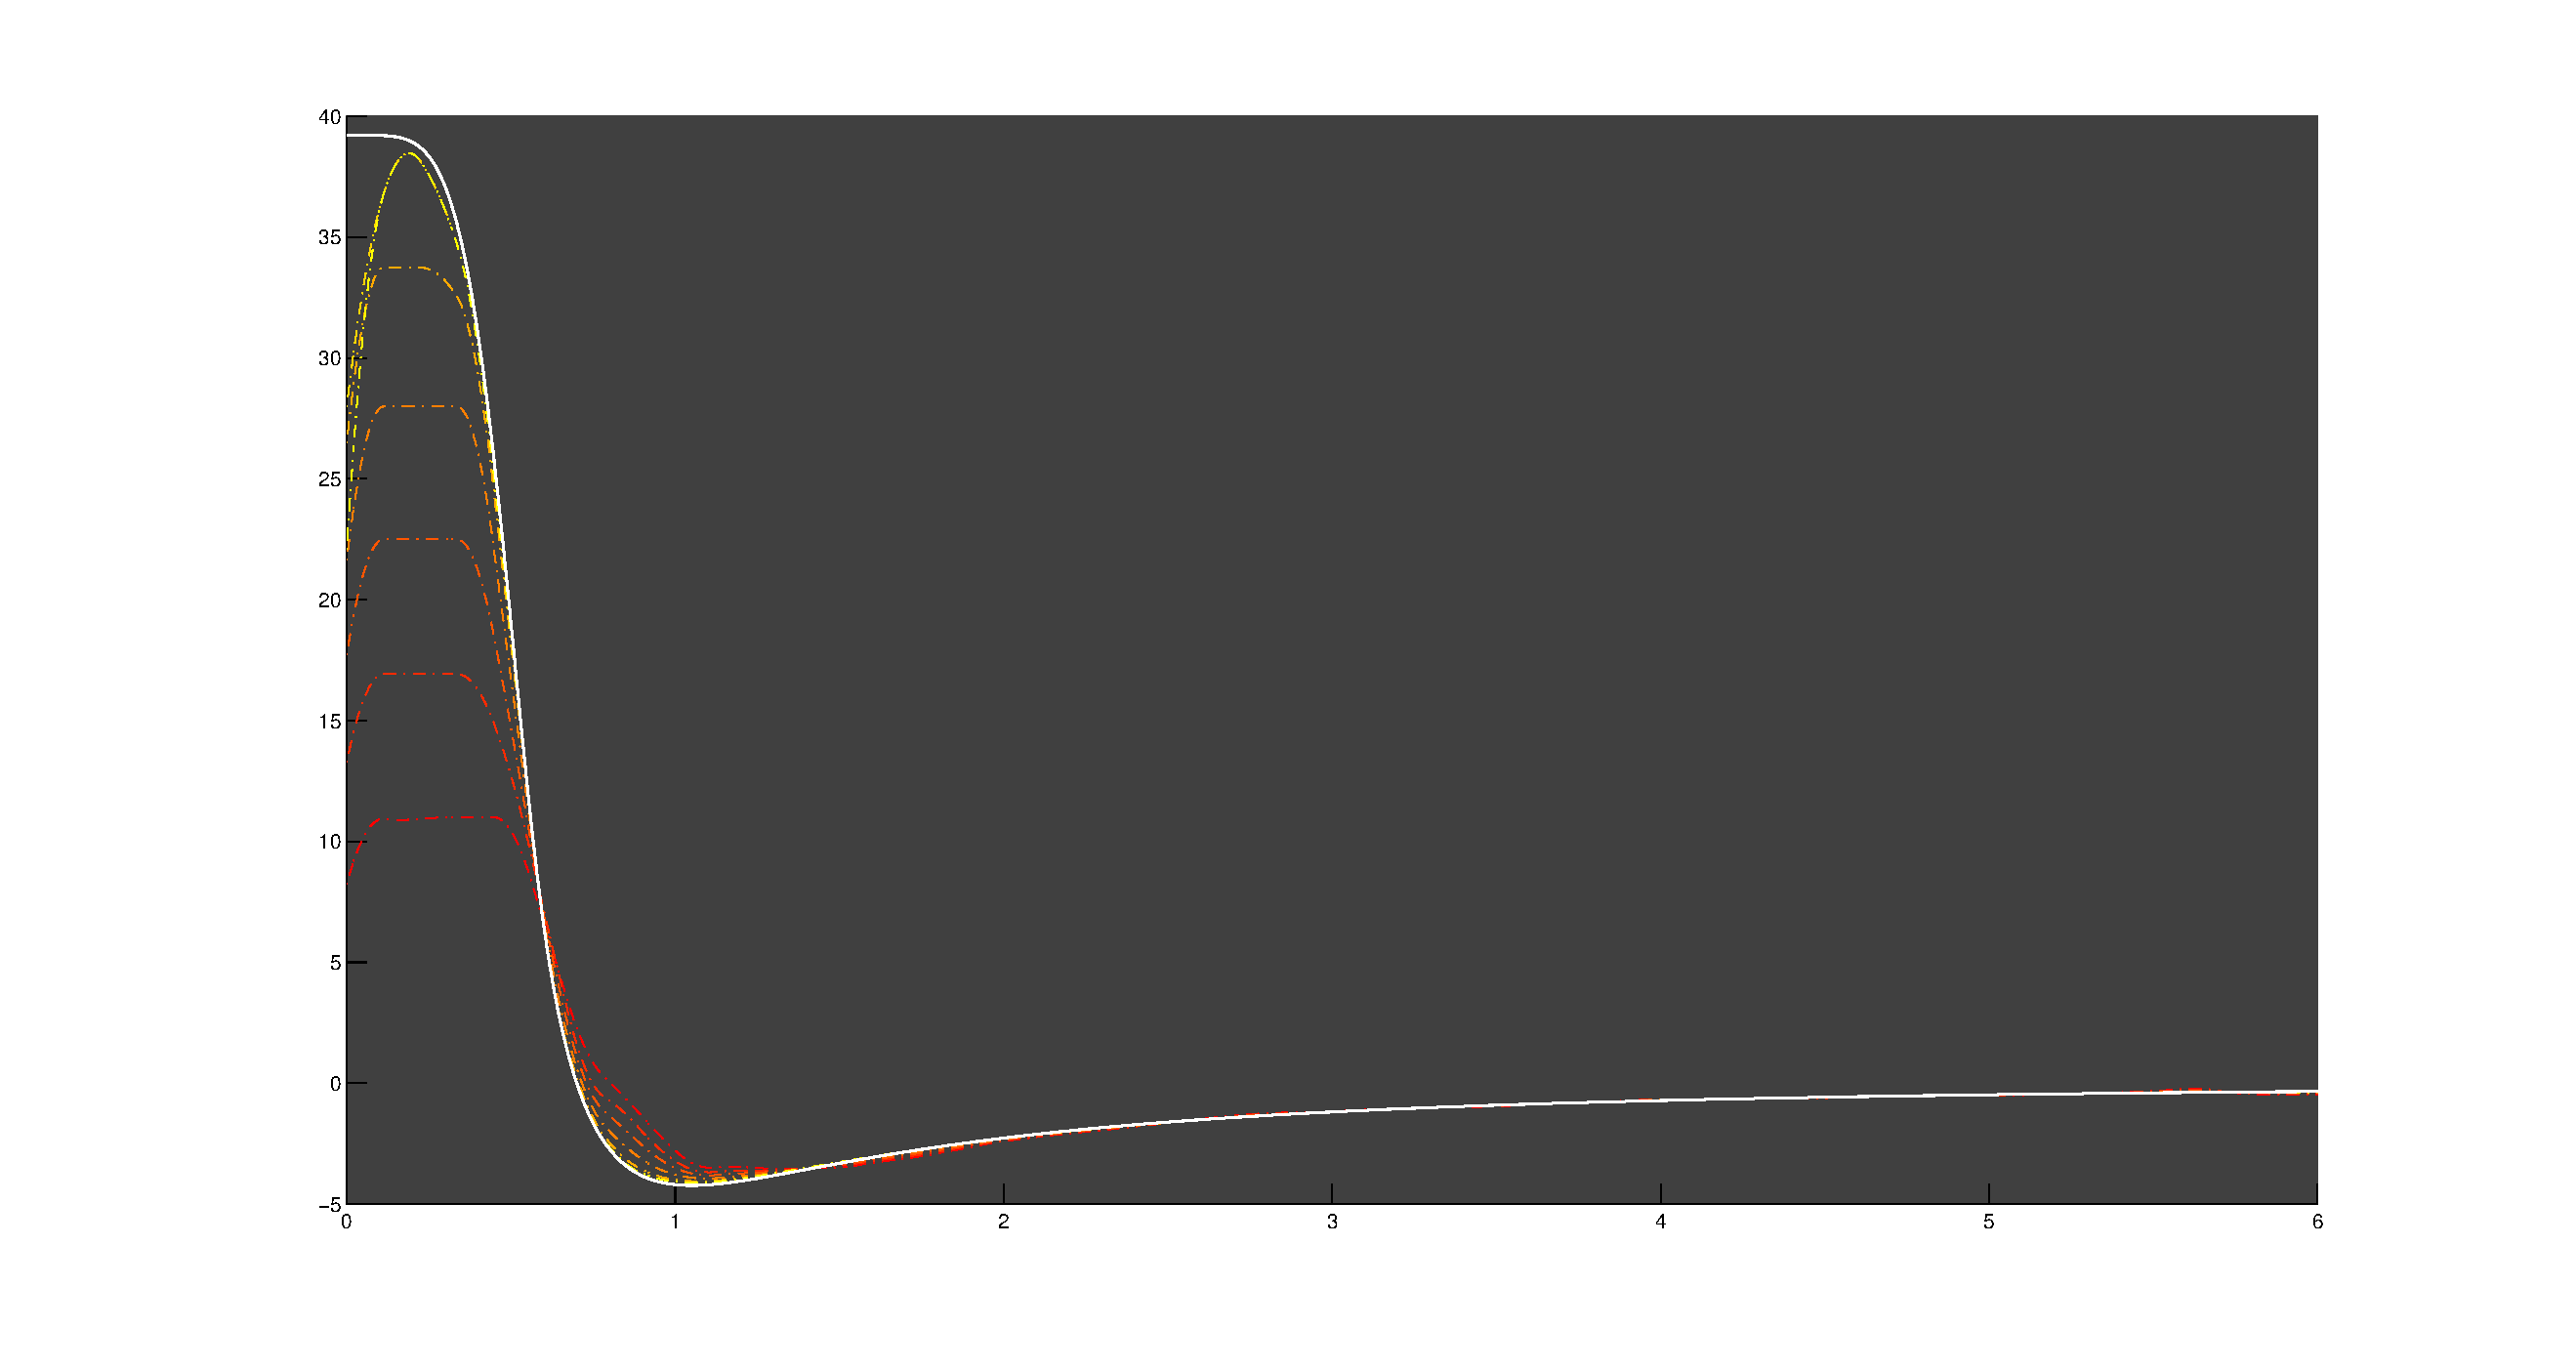
\includegraphics[width=0.53\textwidth]{figPotfun8}
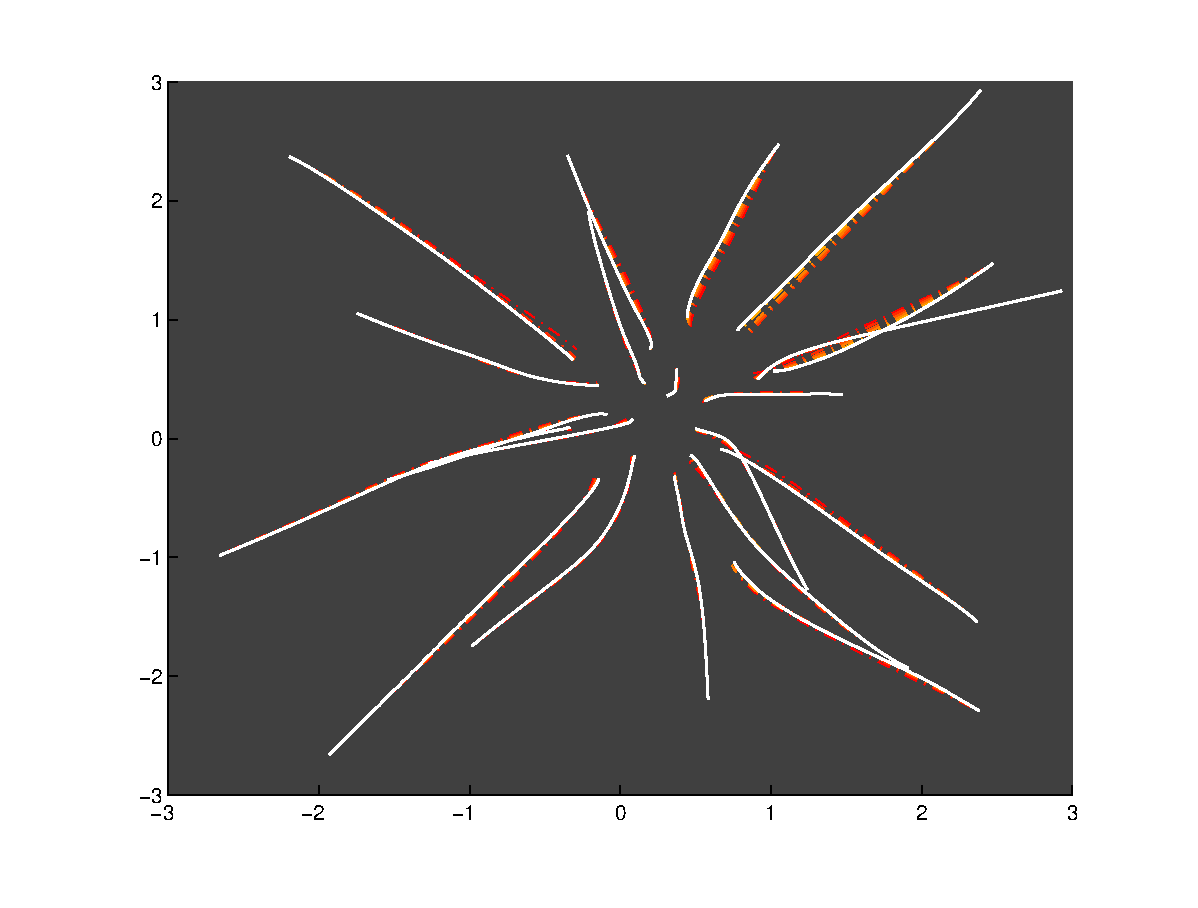
\includegraphics[width=0.37\textwidth]{figTrajfun8}\\
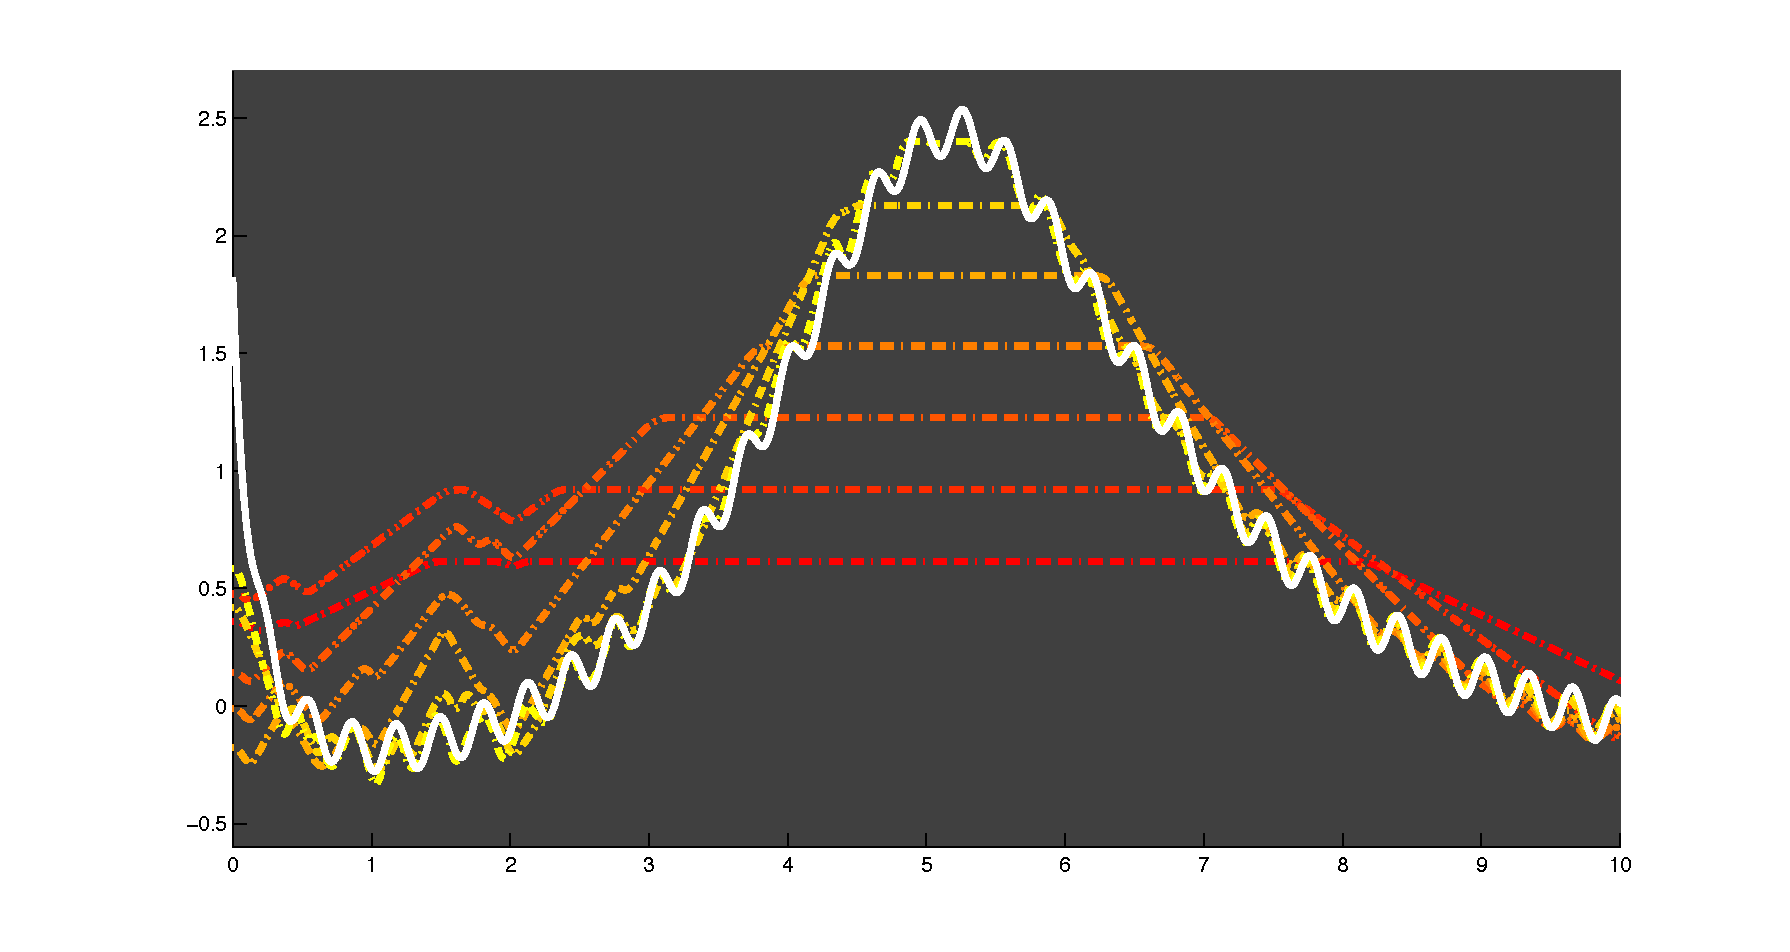
\includegraphics[width=0.53\textwidth]{figPotfun61}
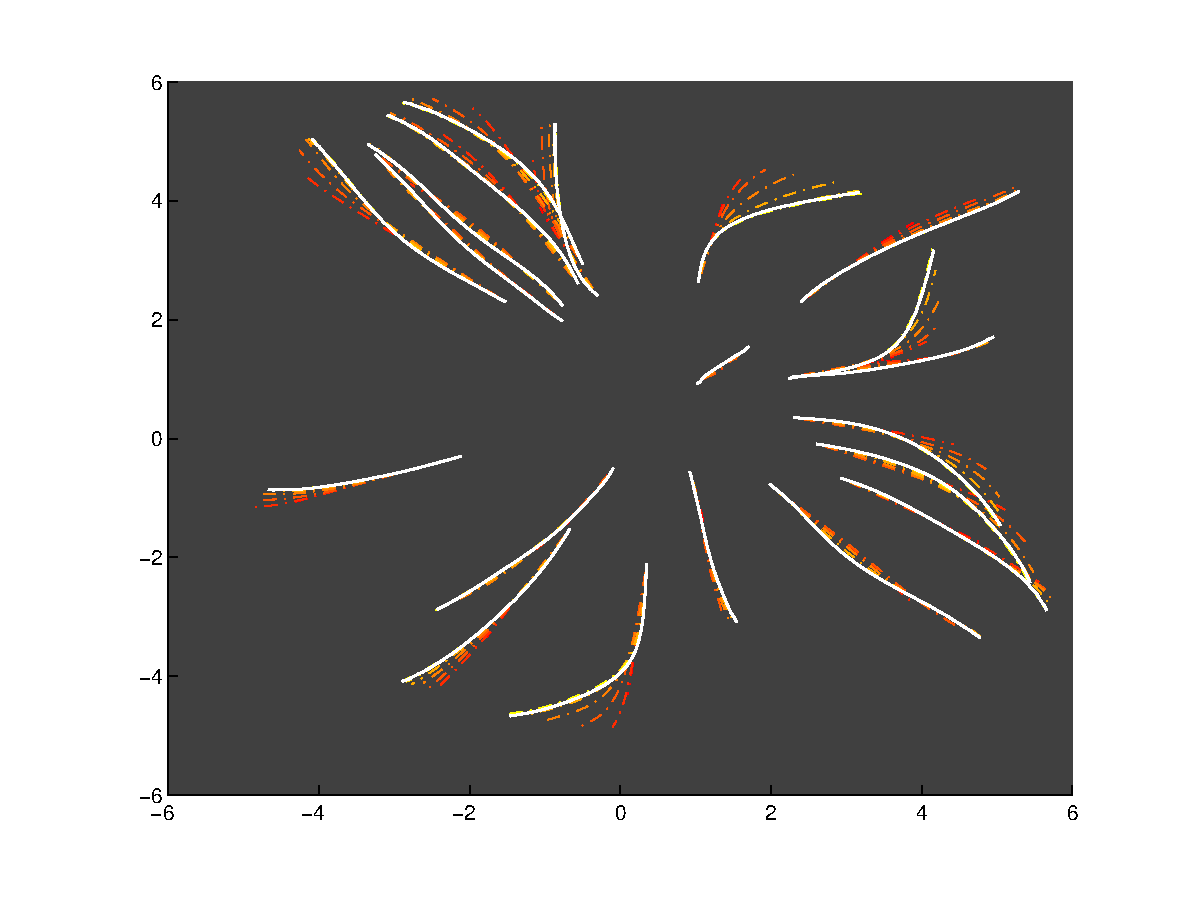
\includegraphics[width=0.37\textwidth]{figTrajfun61}
\end{center}
\caption{Iterative reconstruction of a potential with different values of $M$. On the left column: the true kernel in white and its reconstructions for different $M$; the brighter the curve, the larger the $M$. On the right column: the true trajectories of the agents in white, the trajectories associated to the reconstructed potentials with the same color.\MMcomment{This pictures appear on gray/dark background when I compile, instead of white...}}\label{Mconstr1}
\end{figure}

Until now, we have no criteria to sieve those values of $M$ which enable a successful reconstruction of a potential $a \in X$. To carry out such an analysis, we fix all the parameters of our problem as in Table \ref{tab:fig4} and again take $a$ to be the truncated Lennard-Jones type potential of Figure \ref{variableN}. From what we said in the previous section regarding the continuous-time error functional $\mathcal{E}_N$, we can expect two things from the discrete-time one $\overline{\mathcal{E}}_N$ if we keep $N$ fixed:
\begin{itemize}
\item that $\overline{\mathcal{E}}_N(\widehat{a}_M)$ will be decreasing as $M$ increases. This follows from the fact that our constraint in problem \eqref{problem2} is an inequality, therefore the bigger $M$, the larger the class of potential minimizers;
\item that there is a critical value $\overline{M} > 0$ such that $\overline{\mathcal{E}}_N(\widehat{a}_M)$ stabilizes as $M \geq \overline{M}$. Indeed, from the assumption $a \in X$ follows that after you hit $\overline{M} := \|a\|_{L_{\infty}(K)} + \|a'\|_{L_{\infty}(K)}$, the class of potential minimizers should not grow much more.
\end{itemize}

\begin{table}[h]
\begin{center}
\begin{tabular}{ |c|c|c|c|c|c| }
\hline
  $d$ & $L$ & $T$ & $M$ & $N$ & $D(N)$ \\
\hline
\hline
  $2$ & $3$ & $0.5$ & $[0,10,20,\ldots,200]$ & $50$ & $100$ \\
\hline
\end{tabular}
\end{center}
\vspace{-0.5cm}
\caption{Parameter values for Figure \ref{Mconstr}} \label{tab:fig4} 
\end{table}

Figure \ref{Mconstr} document precisely this expected behavior. This actually suggests that an effective strategy to find a sufficiently good constraint $M$ \textit{a posteriori} is to perform an experiment like the one in Figure \ref{Mconstr} and to choose an $M$ after which the curve of $\overline{\mathcal{E}}_N(\widehat{a}_M)$ flattens.

\subsection{Reconstruction with $N$ fixed}

We now explore the possibility of a reconstruction strategy which does not rely on increasing the value of $N$. Indeed, problem \eqref{problem2} can swiftly become unfeasible when $N$ is moderately large, also because the dimension of the invading subspaces $V_N$ increase with $N$ too. A strategy to overcome this limitation could be to consider, for a fixed $N$, several discrete initial data $(\mu^N_{0,i})_{i = 1}^{\Theta}$ all independently drawn from the same distribution $\mu_0$ (in our case, the $d$-dimensional cube $[-L,L]^d$). For every $i = 1,\ldots,\Theta$, we simulate the system until time $T$ and, with the trajectories we obtain, we solve problem \eqref{problem2}. At the end of this procedure, we have a family of reconstructed potentials $(\widehat{a}_{N,i})_{i = 1}^{\Theta}$, all approximating the same true kernel $a$. Averaging these potentials, we obtain a functional
\begin{align*}
\widehat{a}_N(r) = \frac{1}{\Theta} \sum^{\Theta}_{i = 1}\widehat{a}_{N,i}(r), \quad \text{ for every } r \in [0,R],
\end{align*}
which we claim to be a good approximation to the true kernel $a$. To motivate this claim, we report the outcome of an experiment whose data can be found in Table \ref{tab:fig5}.

\begin{table}[h]
\begin{center}
\begin{tabular}{ |c|c|c|c|c|c|c| }
\hline
  $d$ & $L$ & $T$ & $M$ & $N$ & $D(N)$ & $\Theta$ \\
\hline
\hline
  $2$ & $2$ & $0.5$ & $1000$ & $50$ & $150$ & 5  \\
\hline
\end{tabular}
\end{center}
\vspace{-0.5cm}
\caption{Parameter values for Figure \ref{fixedN}} \label{tab:fig5} 
\end{table}

Figure \ref{fixedN} shows the true potential $a$ and the averaged reconstruction $\widehat{a}_N$. The black-dotted lines corresponds to the 95\% confidence interval obtained from the averaged data.

\begin{figure}[h!]
\begin{center}
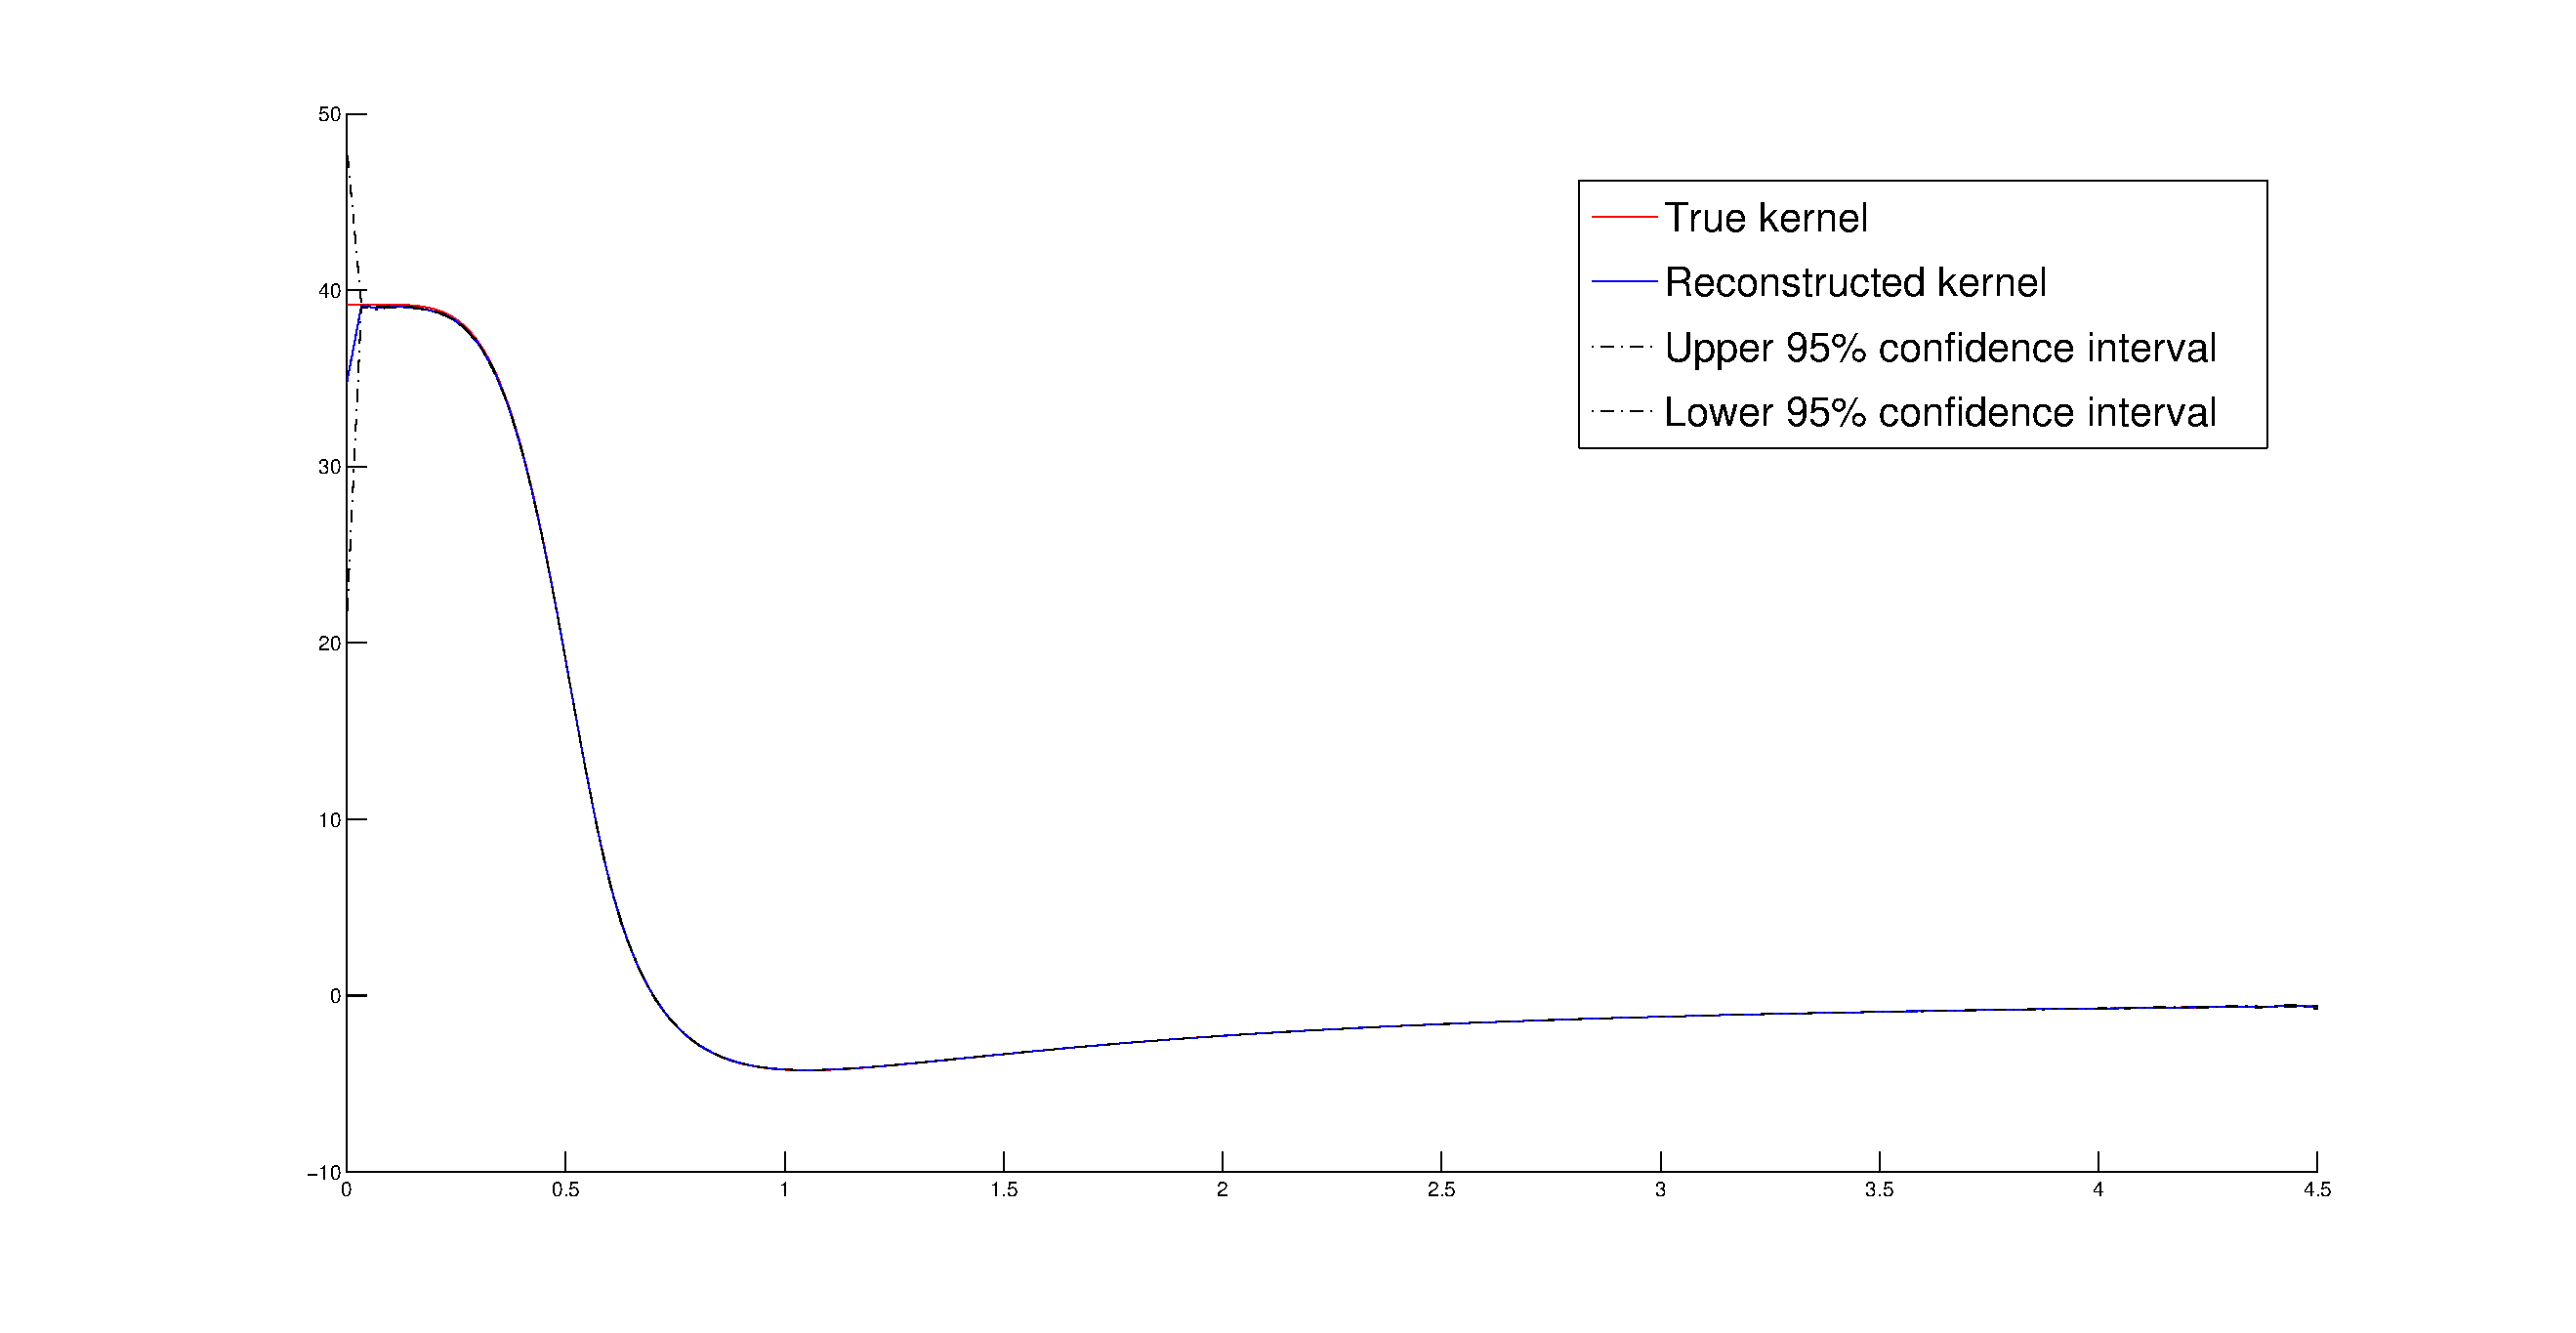
\includegraphics[width=\textwidth]{figNfisso.eps}
\end{center}
\caption{Reconstruction of $a$ obtained by averaging 5 solutions of the minimization of $\mathcal{E}_N$ for $N = 50$. In red: the unknown kernel. In blue: the average of reconstructions. In black: 95\% confidence interval.}\label{fixedN}
\end{figure}